\chapter{实验结果与分析}

\section{评价指标}

\subsection{精度评价指标}
本文使用到的评价目标检测模型精度的指标有精度(Precision)、召回率(Recall)、平均精度(Average Precision, AP)及平均精度均值(mean Average Precision, mAP)。

% IoU用来表示预测框的准确率,它在训练阶段反映的是标注框与预测框的重合程度。例如,用A表示预测目标框,用B表示真实目标框,IoU则是A、B两个框的交集与并集的比值。IoU值越大,代表A、B两个框重叠程度越高。IoU要搭配IoU阈值一起使用。IoU阈值默认被设置为0.5,当两框的IoU大于阈值时,则判断预测框预测正确。
在深度学习中,将分类任务的预测结果分为以下四种,被称作混淆矩阵,见\ref{fig:matrix}:第一种是真正例(True Positive,TP),即模型预测为正例,且实际标签也是正例,预测正确;第二种是假负例(False Negative,FN),指模型预测为负例,但真实标签却是正例,预测错误;第三种是假正例(False Positive,FP),表示模型将负例误判为正例,同样是预测错误;最后一种是真负例(True Negative,TN),即模型预测为负例,同时实际标签也为负例,预测正确。这里的正例和负例其实只是针对某一类别而言的,针对A类而言,A类别就是正例,其他类别就是负例。

精度(Precision)和召回率(Recall),是衡量模型预测准确性与完整性的核心指标。精度的定义如\ref{eq:precision},其中TP表示模型预测为正例,且实际标签也是正例,FP表示模型将负例误判为正例。精度数值越大,表明FP值越小,反映出模型预测结果中真正正例的占比更高,误检更少,预测的准确性更好。召回率(Recall)的定义如\ref{eq:recall},TP同精度公式中的TP,FN表示模型漏掉的正例。召回率数值越大,代表FN值越小,说明模型对实际正例的捕捉能力更强,能够找到更多的正例样本。

% \begin{figure}[!htb]
%     \centering
%     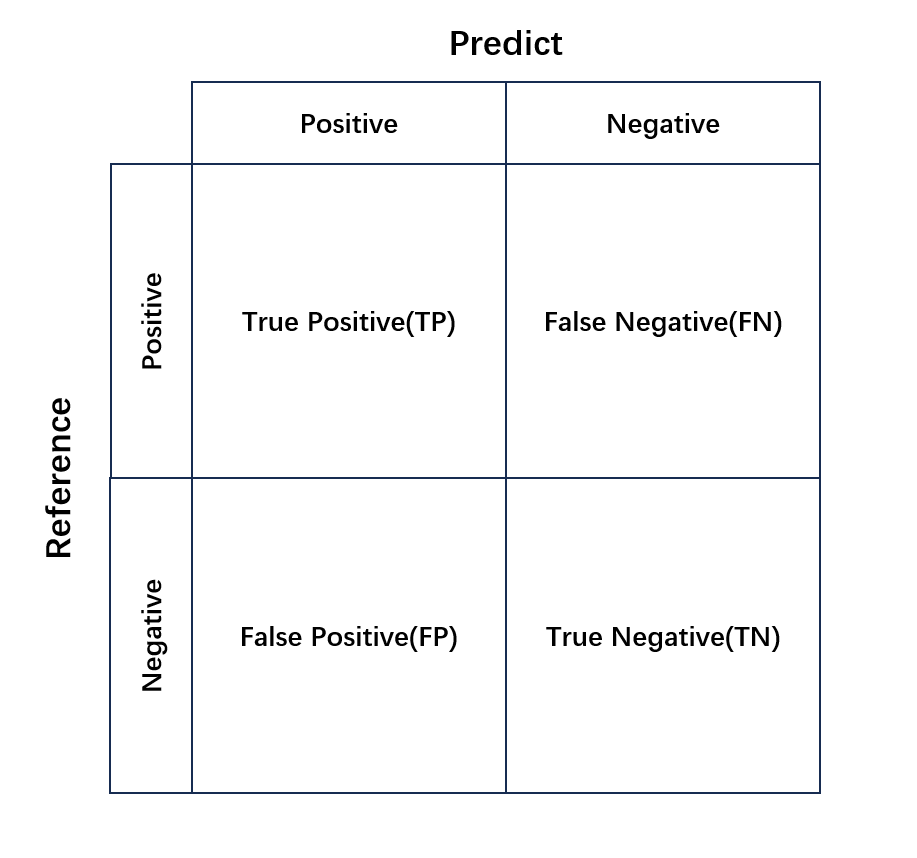
\includegraphics[width=0.6\textwidth]{figs/chap04/matrix.png}
%     \caption{混淆矩阵}
%     \label{fig:matrix}
%   \end{figure}

\begin{equation}
    \begin{aligned}
    Precision = \frac{TP}{TP + FP}\label{eq:precision}
    \end{aligned}
\end{equation}


\begin{equation}
    \begin{aligned}
    Recall = \frac{TP}{TP + FN}\label{eq:recall}
    \end{aligned}
\end{equation}

P-R曲线即为分别以Precision与Recall为坐标围成的曲线,平均精度(AP)通过计算各类别P-R曲线与坐标轴所围成区域的面积来衡量模型性能。从几何意义上讲,若模型的AP值越高,意味着其P-R曲线与坐标轴所围合的区域面积越大,直观反映出该模型在精度(Precision)与召回率(Recall)两个关键指标上的综合表现更好,在整体数据预测中能够同时实现较高的正例预测纯度与正例捕捉能力。平均精度均值(mAP)是对所有类别的AP求平均值,用于反映整个模型的准确率。在YOLO模型中,常见的mAP评价指标有mAP50和mAP50-95。mAP50为IoU阈值设为0.5时,所有类别的平均精度均值。mAP50-95为IoU阈值从0.5到0.95(间隔0.05递增)的多个严格标准下,分别计算mAP,再取平均值。

% \begin{figure}[!htb]
%     \centering
%     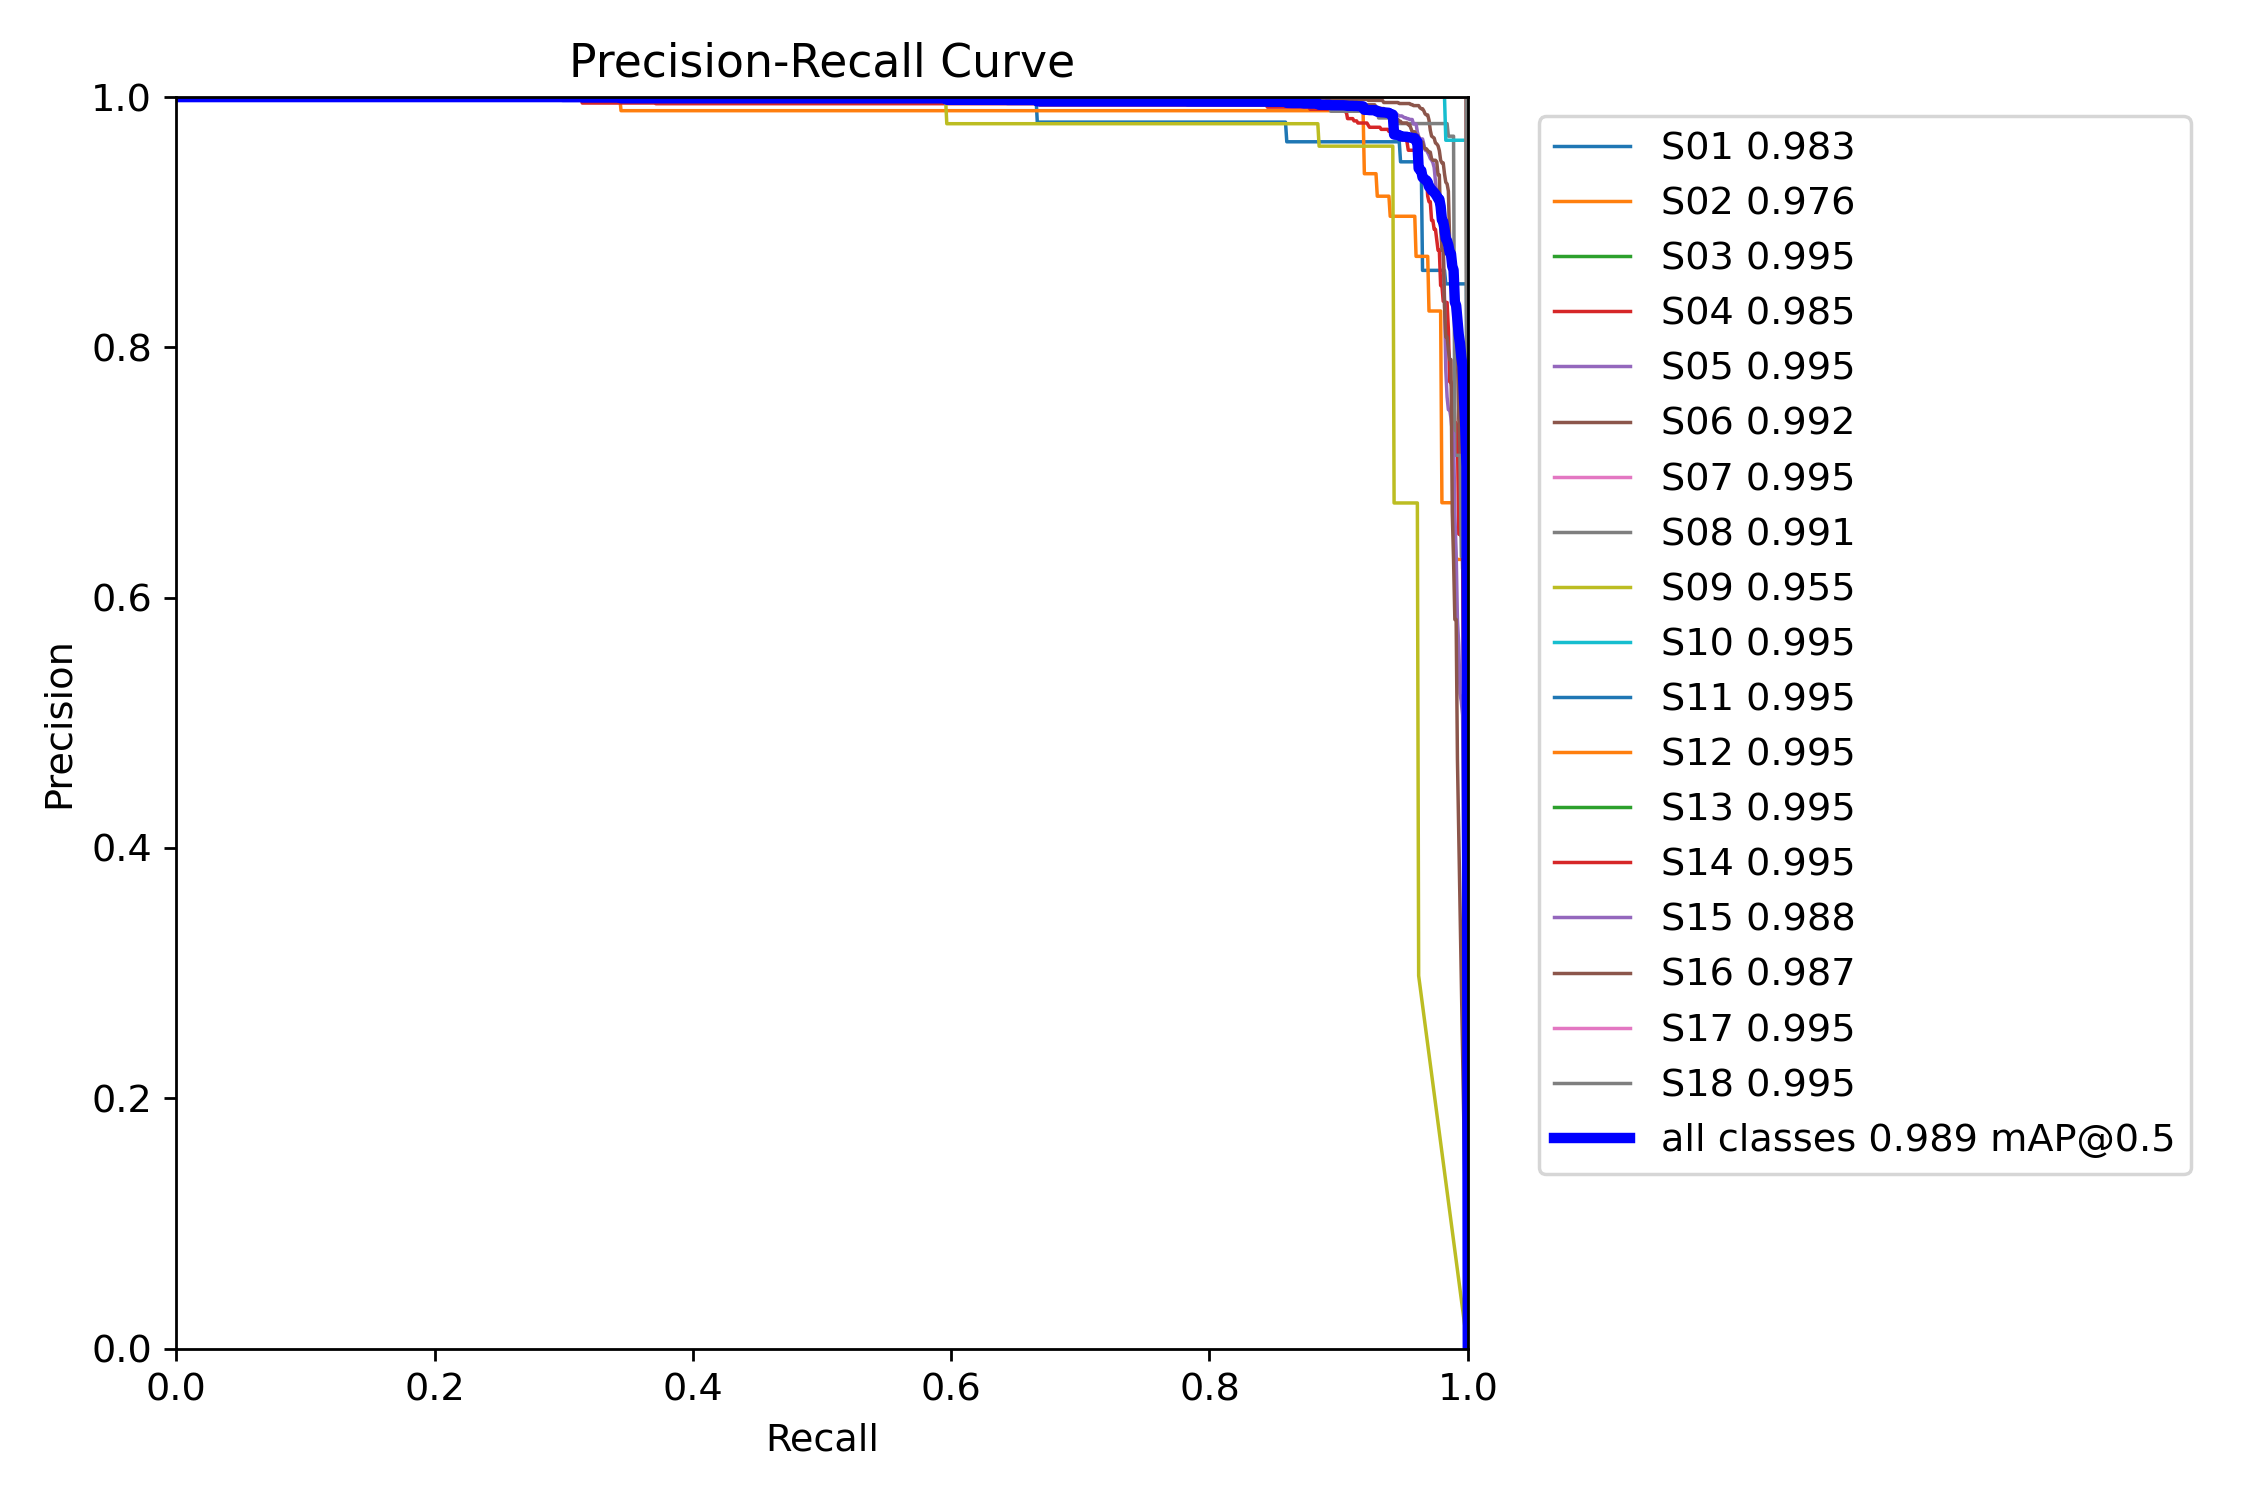
\includegraphics[width=0.6\textwidth]{figs/chap04/PR_curve.png}
%     \caption{PR曲线}
%     \label{fig:pr}
%   \end{figure}

\subsection{速度评价指标}
本文使用到的评价目标检测模型速度的指标有每秒帧率和FLOPs。每秒帧率(Frame Per Second,FPS),即每秒内可以处理的图片数量,能够衡量模型的实时性,FPS越高,实时性越强。FLOPs表示浮点运算量,它衡量了模型在进行一次前向传播(推理)过程中所执行的浮点运算次数,FLOPs越低,理论速度越快,但并不直接等于实际速度。

\section{实验结果分析}
\subsection{头盔佩戴情况模型}
本文基于YOLOv11n、YOLOv11s和YOLOv11m三个模型,各训练了300个epoch,头盔佩戴情况模型训练结果如\ref{fig:helmetResult}所示。下面对边界框回归损失(box\_loss)、分类损失(cls\_loss)、分布损失(dfl\_loss)、精度(precision)、召回率(recall)、mAP50和mAP50-95这七个指标进行详细对比分析。

\begin{figure}[H]
    \centering
    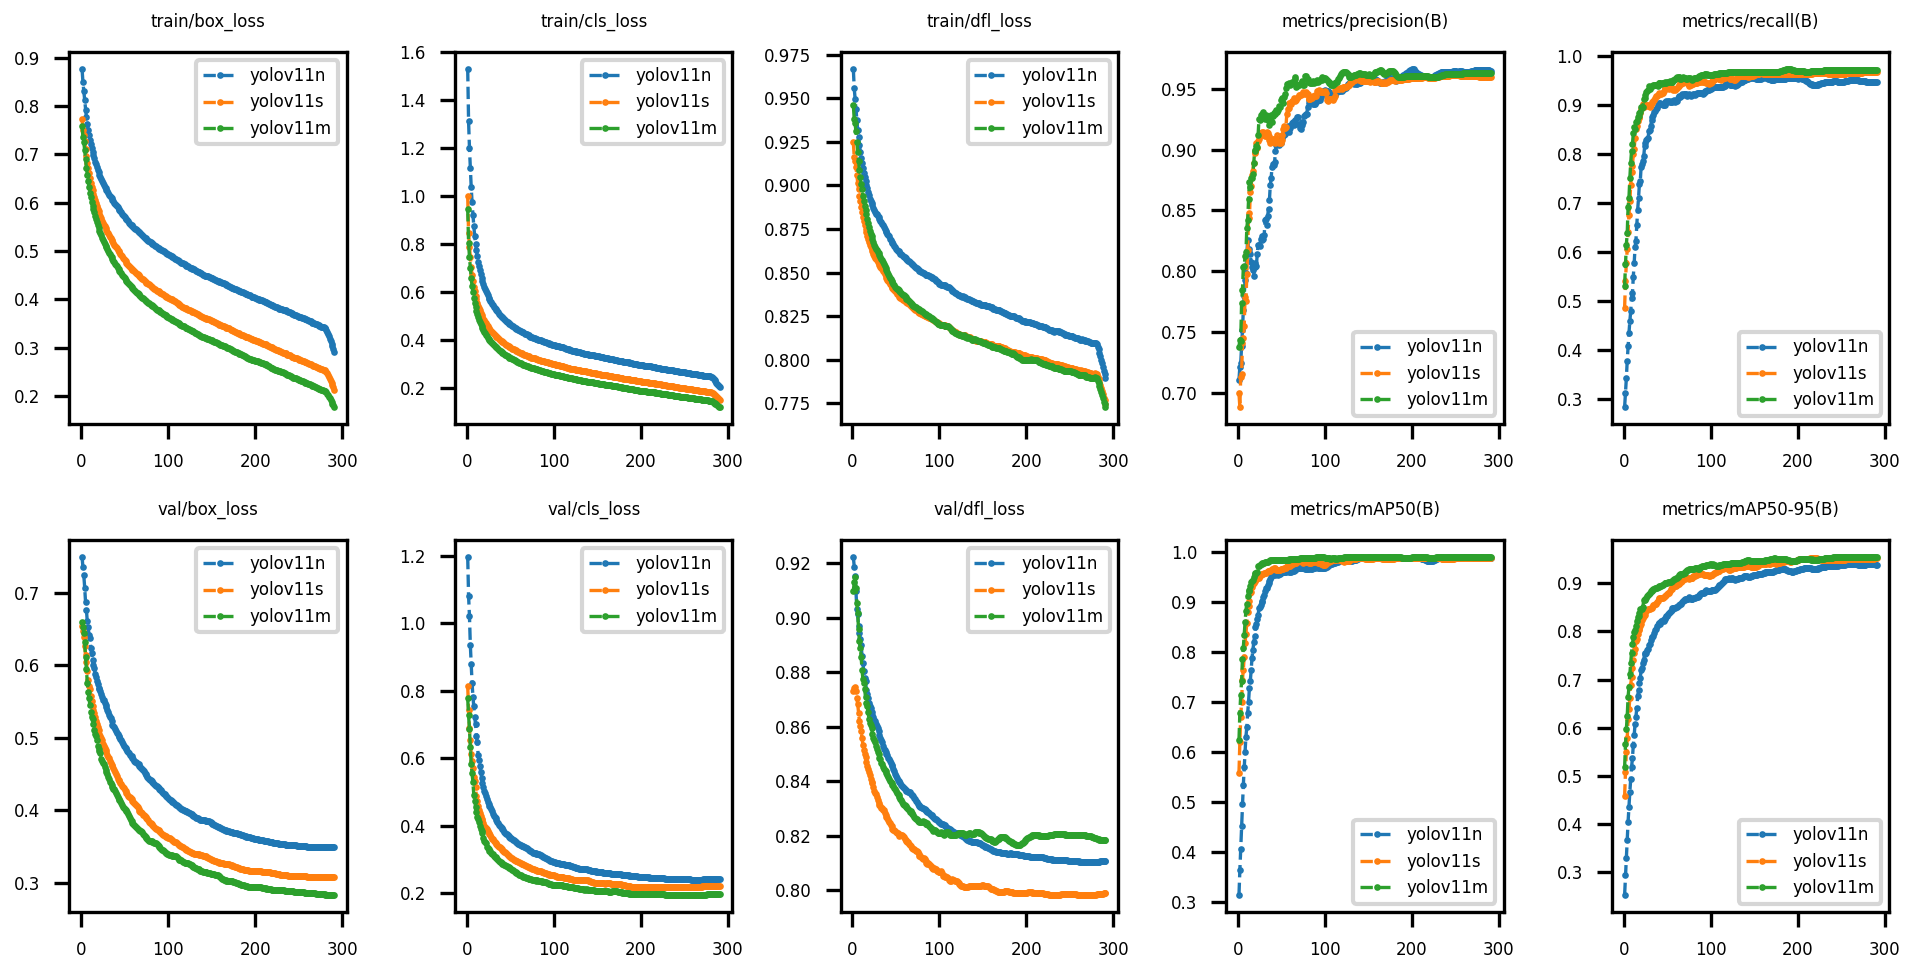
\includegraphics[width=1\textwidth]{figs/chap04/helmetResult.png}
    \caption{头盔佩戴情况模型训练结果}
    \label{fig:helmetResult}
\end{figure}

边界框回归损失:三个模型的边界框回归损失值均随训练轮数的增加呈现下降趋势。YOLOv11n下降趋势相对较缓,YOLOv11s和YOLOv11m前期下降速度较快且相近,在训练进行大约50轮之后,YOLOv11m下降速度略快于YOLOv11s,说明YOLOv11m在边界框回归损失的收敛上最具优势。在训练后期,YOLOv11m的边界框回归损失最终值最低,YOLOv11s次之,YOLOv11n相对较高。这表明YOLOv11m在边界框定位的准确性上表现更好。

分类损失:三个模型分类损失收敛趋势相似,均在前期快速下降,后期平稳下降。前期YOLOv11n下降稍快,YOLOv11s与YOLOv11m相近。中期YOLOv11s和YOLOv11m的下降速度与YOLOv11n相似,后期三者收敛速度相近。
YOLOv11m最终的分类损失值最低,YOLOv11s和YOLOv11n相对较高且较为接近,意味着YOLOv11m在分类任务上的准确性更高。

分布损失:YOLOv11s与YOLOv11m整体收敛趋势相似,前期都比YOLOv11n收敛速度略快,后期三者收敛速度近似。YOLOv11s与YOLOv11m达到的最优值近乎相同,且都比YOLOv11n的最优质更好。

精度:三个模型精度均随训轮数增多呈上升趋势。YOLOv11s和YOLOv11m前期上升速度较快且相近,YOLOv11n稍慢;后期三者趋势相似。YOLOv11m达到的精度最优值最高,YOLOv11s次之,YOLOv11n相对较低,表明YOLOv11m在预测准确程度上表现更优。

召回率:YOLOv11s与YOLOv11m前期收敛趋势相同且均比YOLOv11n收敛速度快;后期三者都逐渐趋于平稳。YOLOv11m召回率最优值最高,YOLOv11s与之接近,YOLOv11n相对较低。说明YOLOv11m在捕捉正例样本能力上表现最好。

mAP50:YOLOv11s和YOLOv11m的mAP50值在训练前期上升迅速,YOLOv11n稍慢;中后期YOLOv11m率先趋于稳定,YOLOv11s次之。三个模型的mAP50最优值近似,意味着三者在IoU阈值为0.5时平均精度近似。

mAP50-95:YOLOv11s和YOLOv11m前期收敛速度快且相近,YOLOv11n比较缓慢;后期YOLOv11m收敛更平稳,更快达到较高精度水平。YOLOv11m的mAP50-95最优值最高,YOLOv11s与之相近,YOLOv11n较低。表明YOLOv11m与YOLOv11s在不同IoU阈值下平均精度综合表现都比较好。

根据训练结果中的csv文件,能够得到各项指标在每一轮训练中的精确值,上述指标在训练过程中的最优值的对比如\ref{tab:modelCompare1}所示。从表格呈现的趋势来看,随着模型规模增大,三个损失函数的收敛速度更快,最终达到的损失值更低。其余四项指标,除检测精度外,召回率、mAP50和mAP50-95三项指标都随模型规模增大表现更优。

\begin{table}[htb]
    \centering
    \caption[目标数据]{模型损失函数与检测精度指标对比1\label{tab:modelCompare1}}
    \begin{tabular}{lccccccc}
        \toprule
        Model & 
        \makecell{box\_loss\\(\%)} & 
        \makecell{cls\_loss\\(\%)} & 
        \makecell{dfl\_loss\\(\%)} & 
        \makecell{Precision\\(\%)} & 
        \makecell{Recall\\(\%)} & 
        \makecell{mAP50\\(\%)} & 
        \makecell{mAP50-95\\(\%)} \\
        \midrule
        YOLOv11n & 28.4 & 20.2 & 78.6 & 96.7 & 96.6 & 99.0 & 94.1 \\
        YOLOv11s & 20.5 & 14.7 & 77.2 & 96.2 & 97.2 & 99.0 & 95.4 \\
        YOLOv11m & 17.1 & 11.8 & 77.1 & 97.3 & 98.1 & 99.1 & 95.5 \\
        \bottomrule
    \end{tabular}
\end{table}


除了检测精度,模型的推理速度与计算复杂度同样是衡量性能的关键要素,\ref {tab:speedCompare1}对比了YOLOv11n、YOLOv11s和YOLOv11m三个版本基于实测数据的FPS与FLOPs数值。对于FPS指标,YOLOv11n的值最高,达到41.67,意味着该模型每秒能够处理41.67帧图像,实时性最强;YOLOv11s的FPS为36.63,仅次于YOLOv11n;YOLOv11m的FPS最低,为31.75。由此可见,随着模型规模增大(从n到m),检测速度逐渐降低,因为更大的模型通常包含更多的参数和计算操作,需要更长的推理时间。对于FLOPs指标,YOLOv11m的FLOPs值最高,为68.26G,表明其完成一次前向推理所需的浮点运算次数最多,计算复杂度最高;YOLOv11s的FLOPs为21.59G;而YOLOv11n的 FLOPs最低,仅为6.4G。综合两项指标来看,YOLOv11模型的检测精度与计算速度呈现负相关性。YOLOv11n在检测精度上略逊于其他版本,但其计算复杂度低、检测速度快;而YOLOv11m推理速度较慢,但其在复杂场景下具有更高的检测精度。

\begin{table}[htb]
    \centering
    \caption[目标数据]{模型检测速度对比1\label{tab:speedCompare1}}
    \begin{tabular}{lcc}
        \toprule
        Model & 
        \makecell{FPS(1)} & 
        \makecell{FLOPs(G)} \\
        \midrule
        YOLOv11n & 41.67 & 6.4 \\
        YOLOv11s & 36.63 & 21.59 \\
        YOLOv11m & 31.75 & 68.26 \\
        \bottomrule
    \end{tabular}
\end{table}

% 6.46G 21.59G 68.26G   24 27.3 31.5

三个模型的混淆矩阵如\ref{fig:nmatrix}、\ref{fig:smatrix}、\ref{fig:mmatrix}所示。YOLOv11n对S07类别的检测效果较差,有33\%的错误预测情况。对S09类别有6\%的误判和6\%的漏检。对剩余标签的检测准确度都在94\%以上。YOLOv11s相较于YOLOv11n,对S07和S09两个标签的检测准确度有大幅提升,且对所有标签的检测精度都在94\%以上。YOLOv11m相较于YOLOv11n,对各类别的检测精度近似,没有大幅变化,且对所有标签的检测精度也都在94\%以上。

\begin{figure}[H]
    \centering
    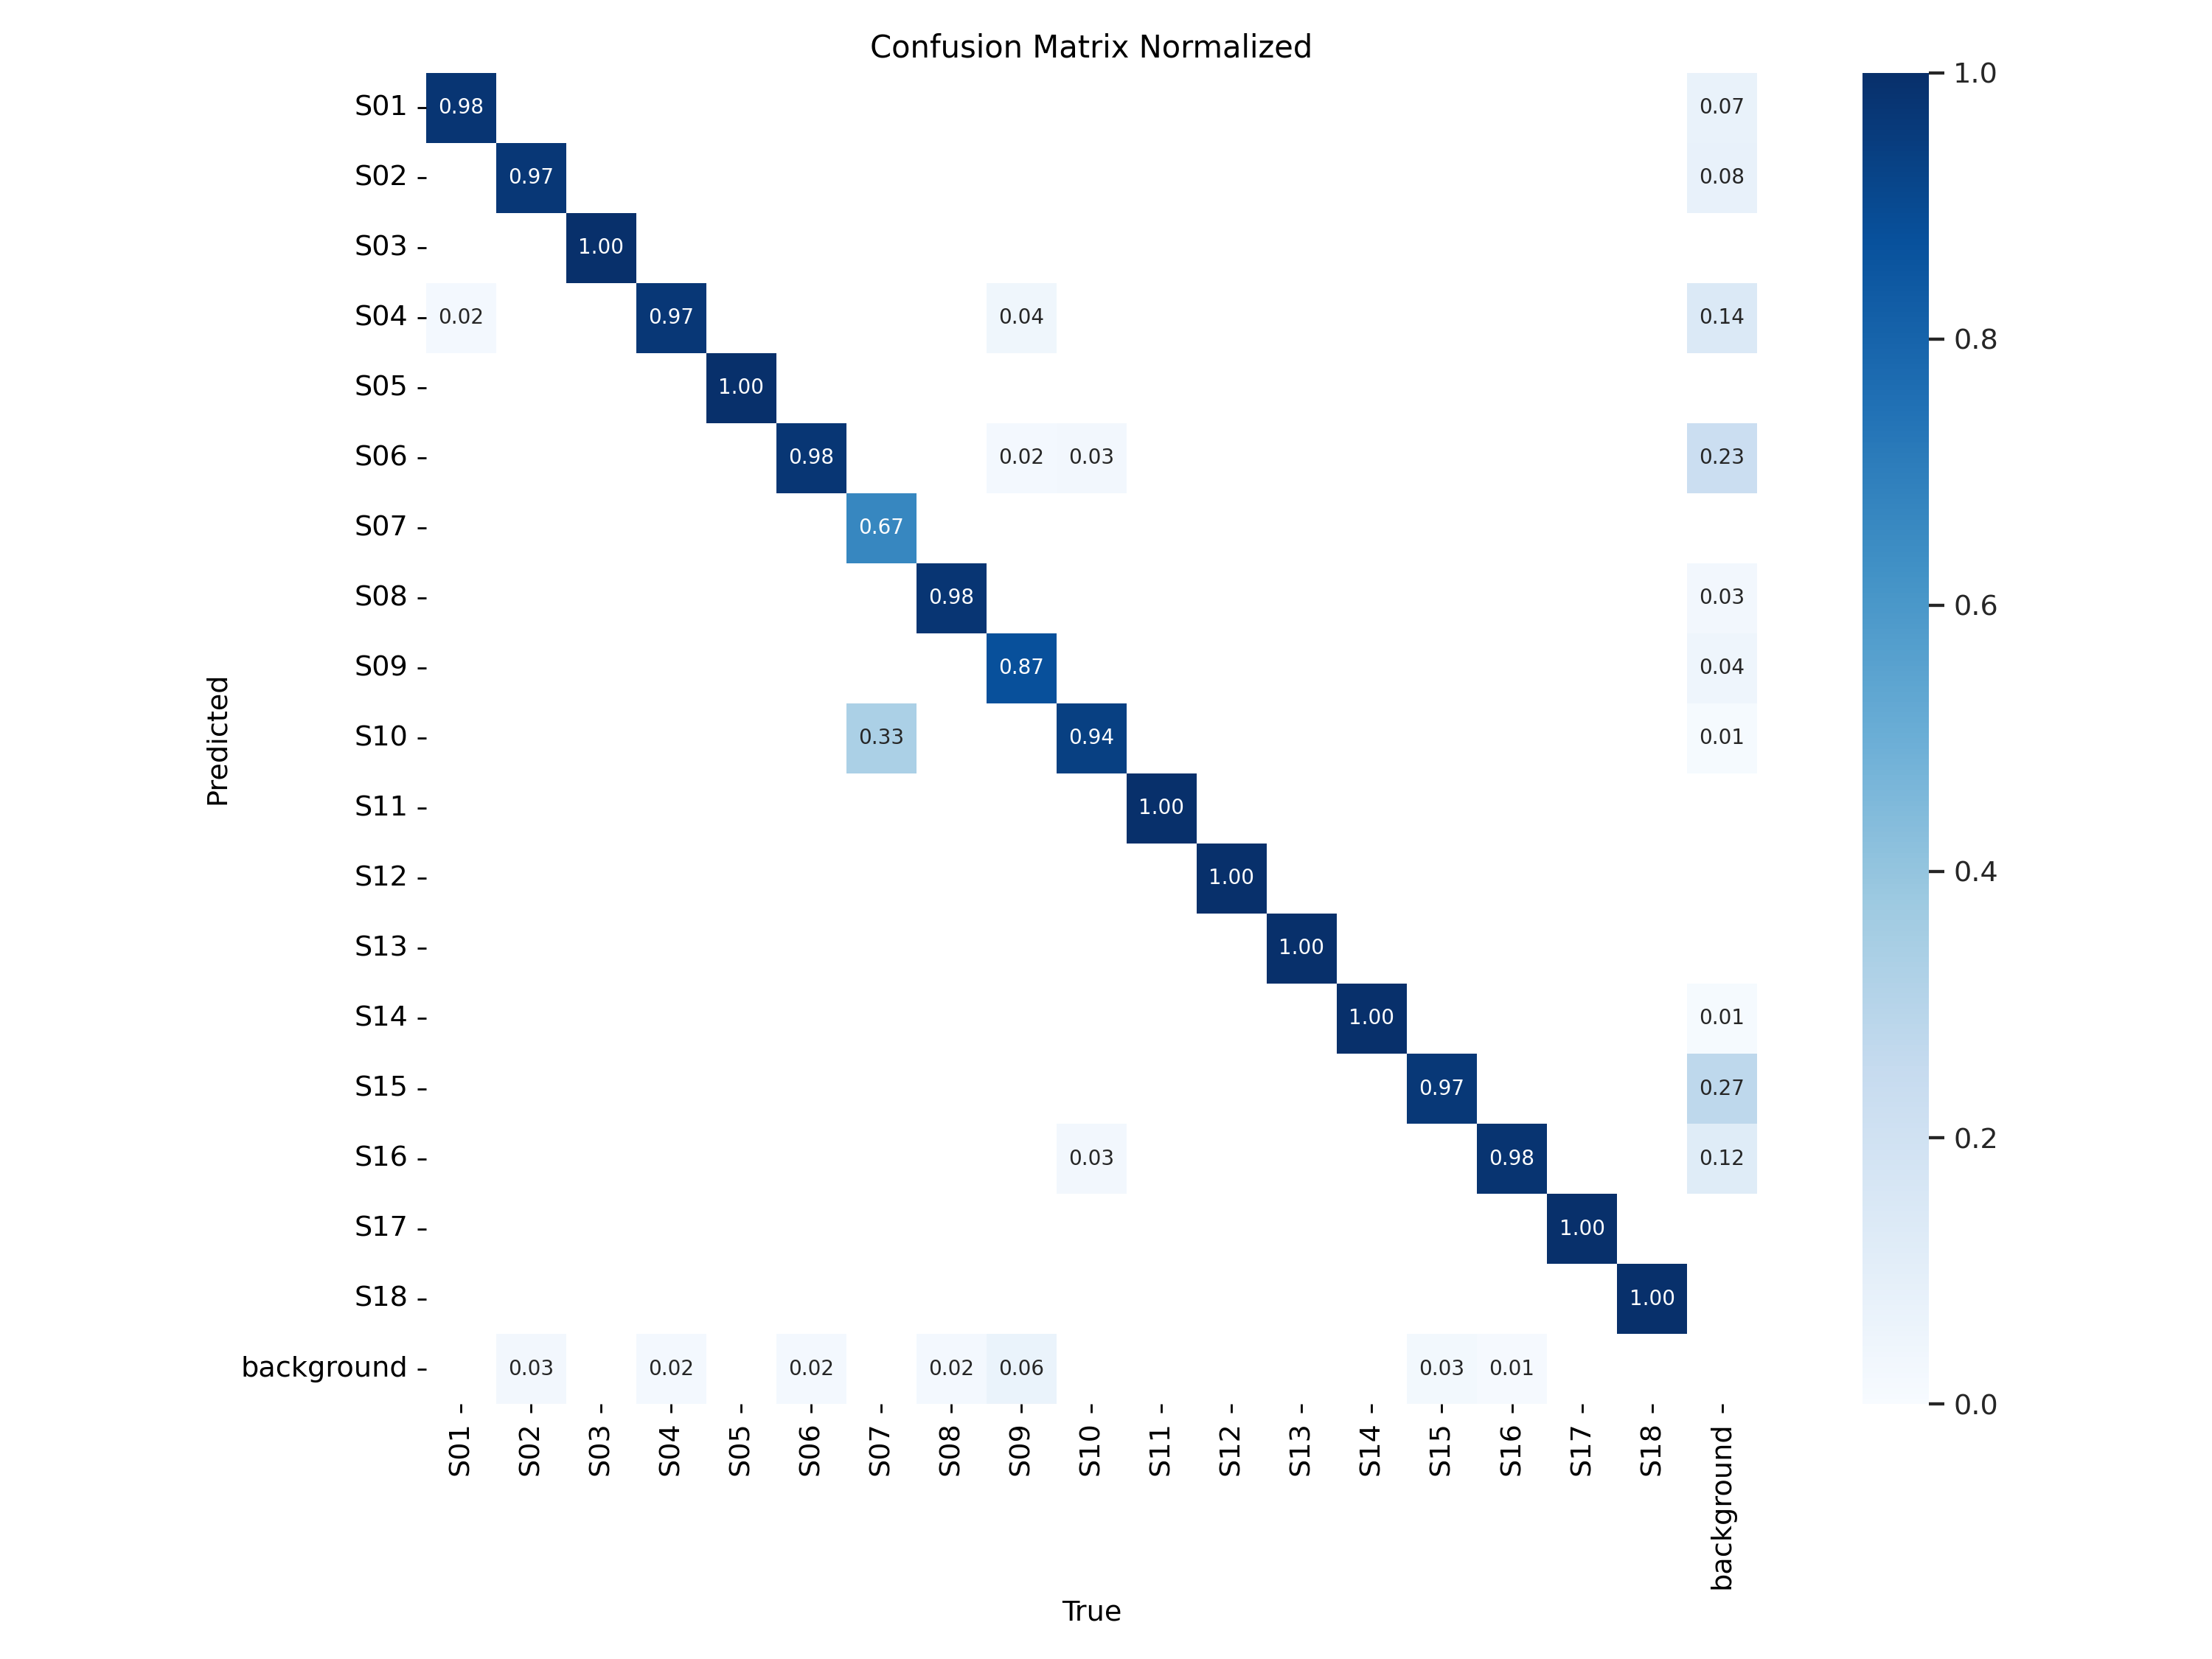
\includegraphics[width=0.85\textwidth]{figs/chap04/n_confusion_matrix_normalized.png}
    \caption{YOLOv11n混淆矩阵}
    \label{fig:nmatrix}
\end{figure}


\begin{figure}[h]
    \centering
    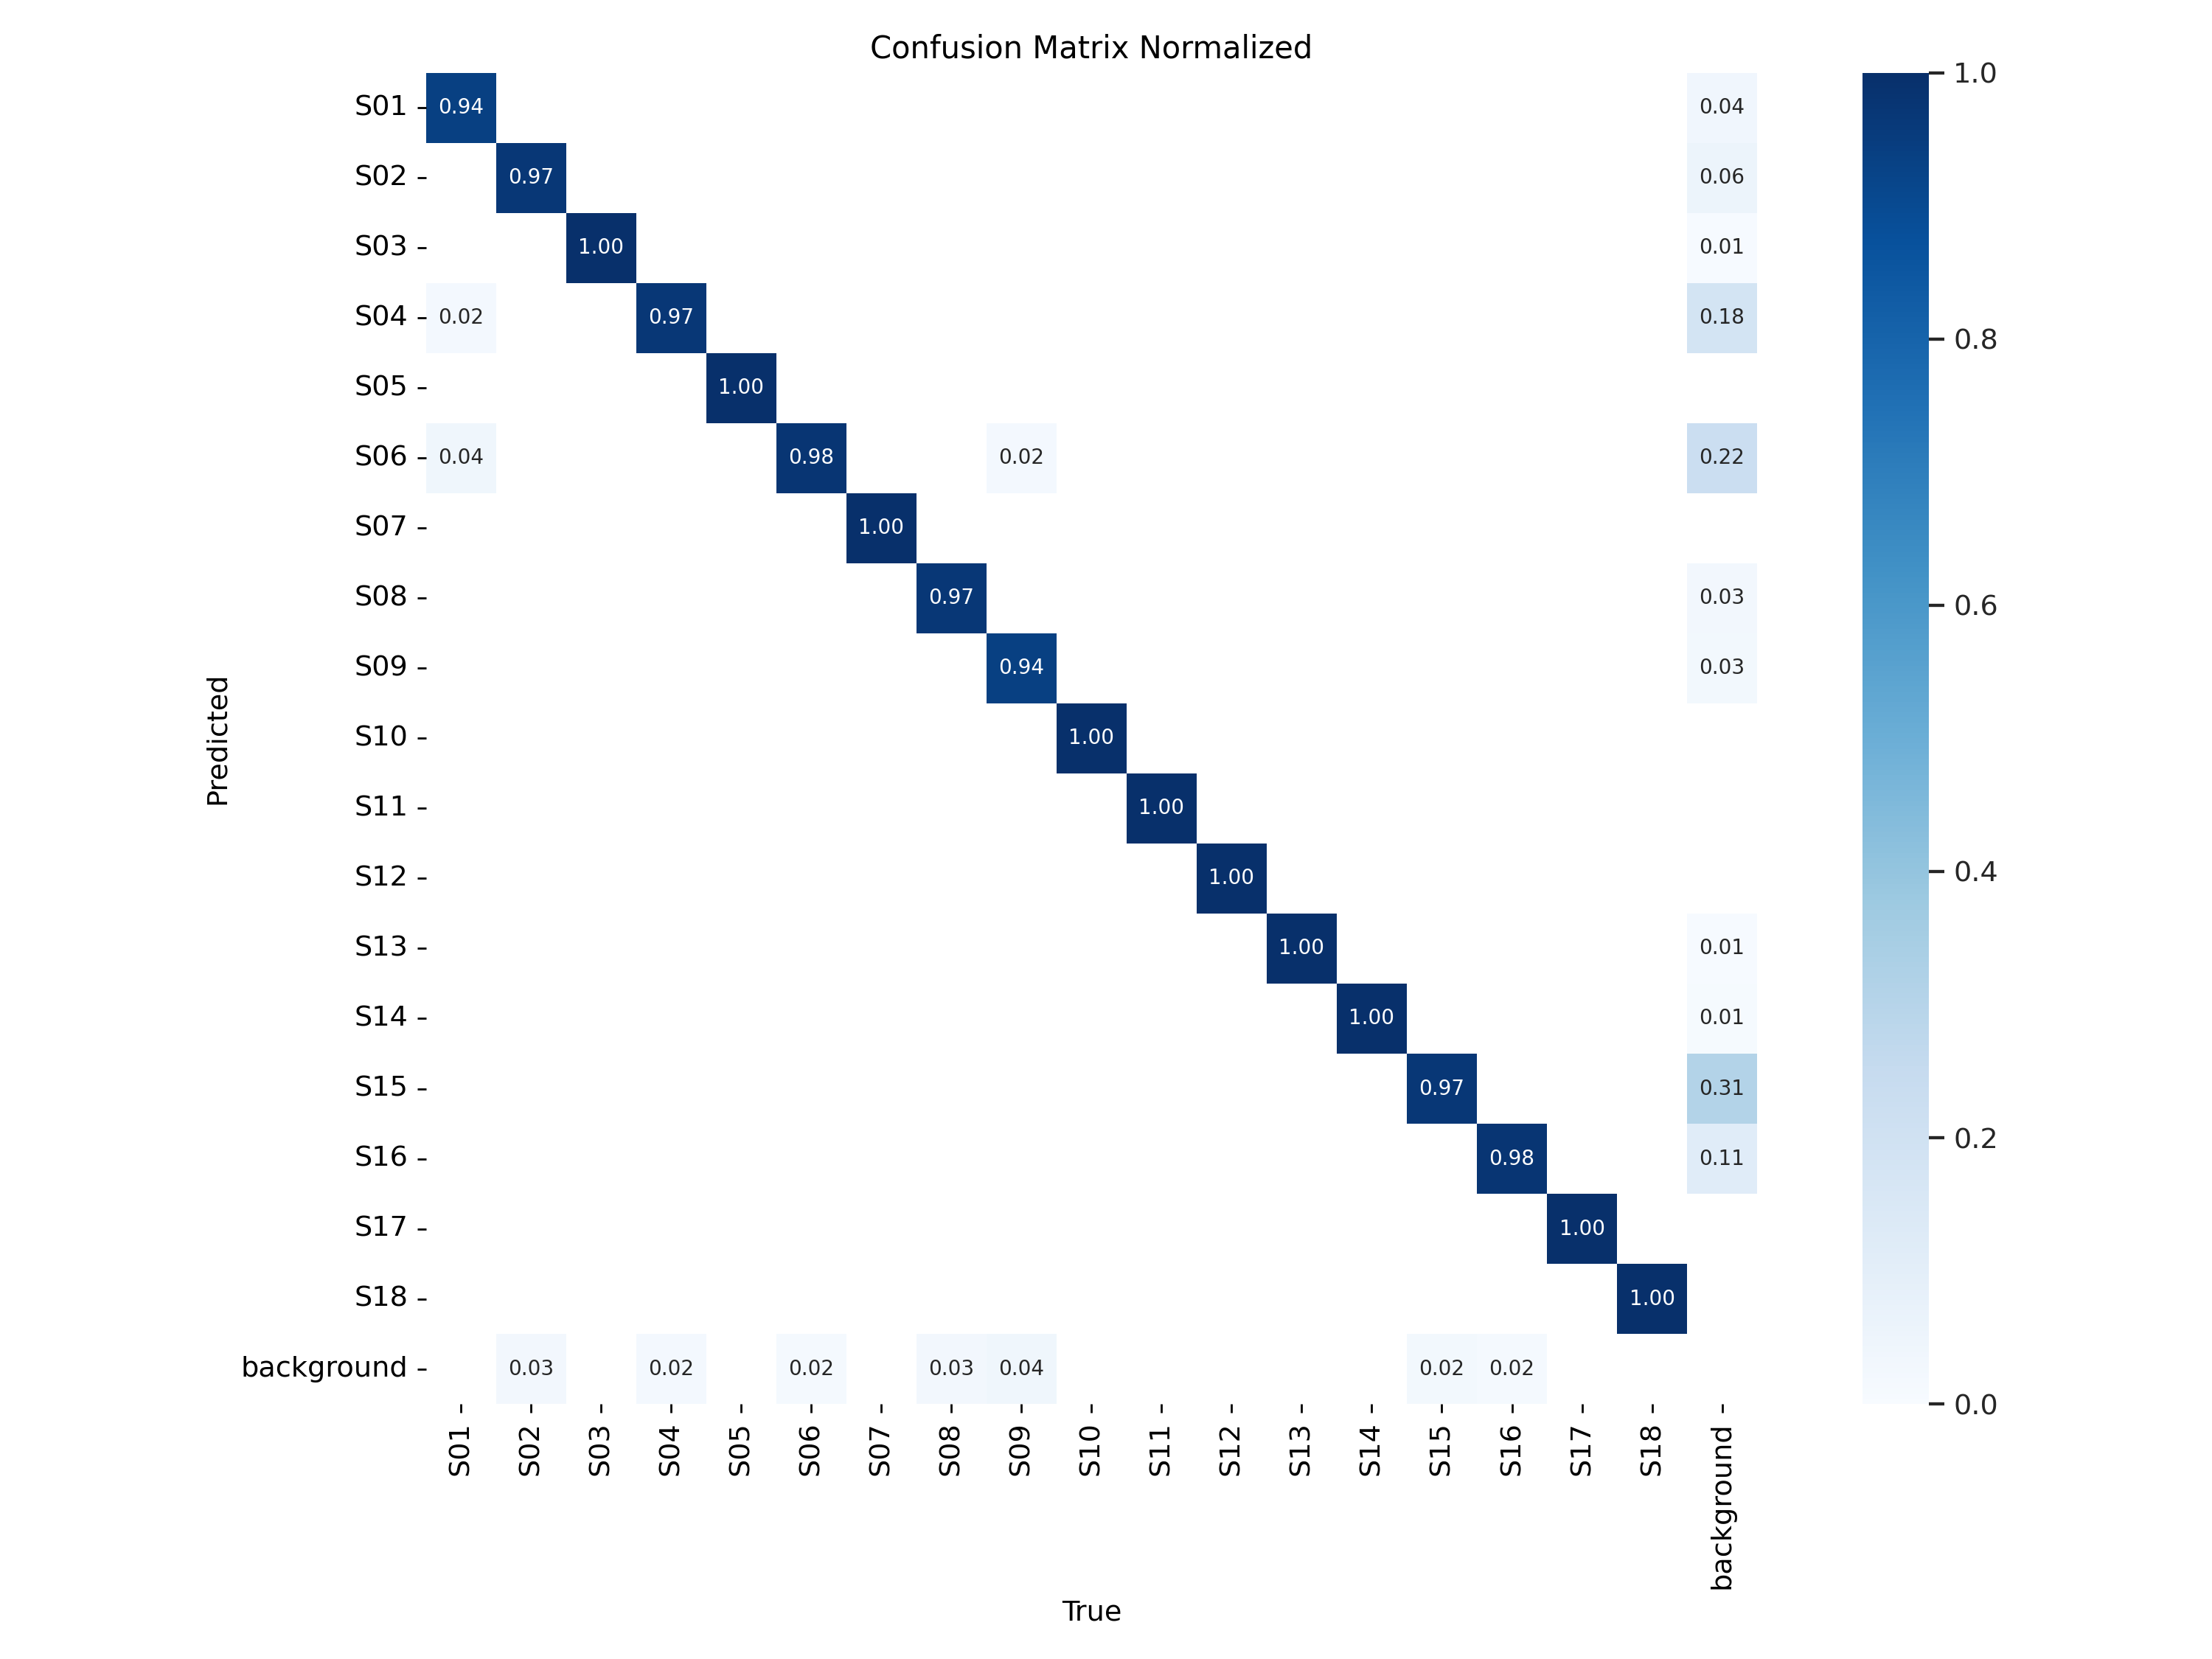
\includegraphics[width=0.85\textwidth]{figs/chap04/s_confusion_matrix_normalized.png}
    \caption{YOLOv11s混淆矩阵}
    \label{fig:smatrix}
\end{figure}


\begin{figure}[H]
    \centering
    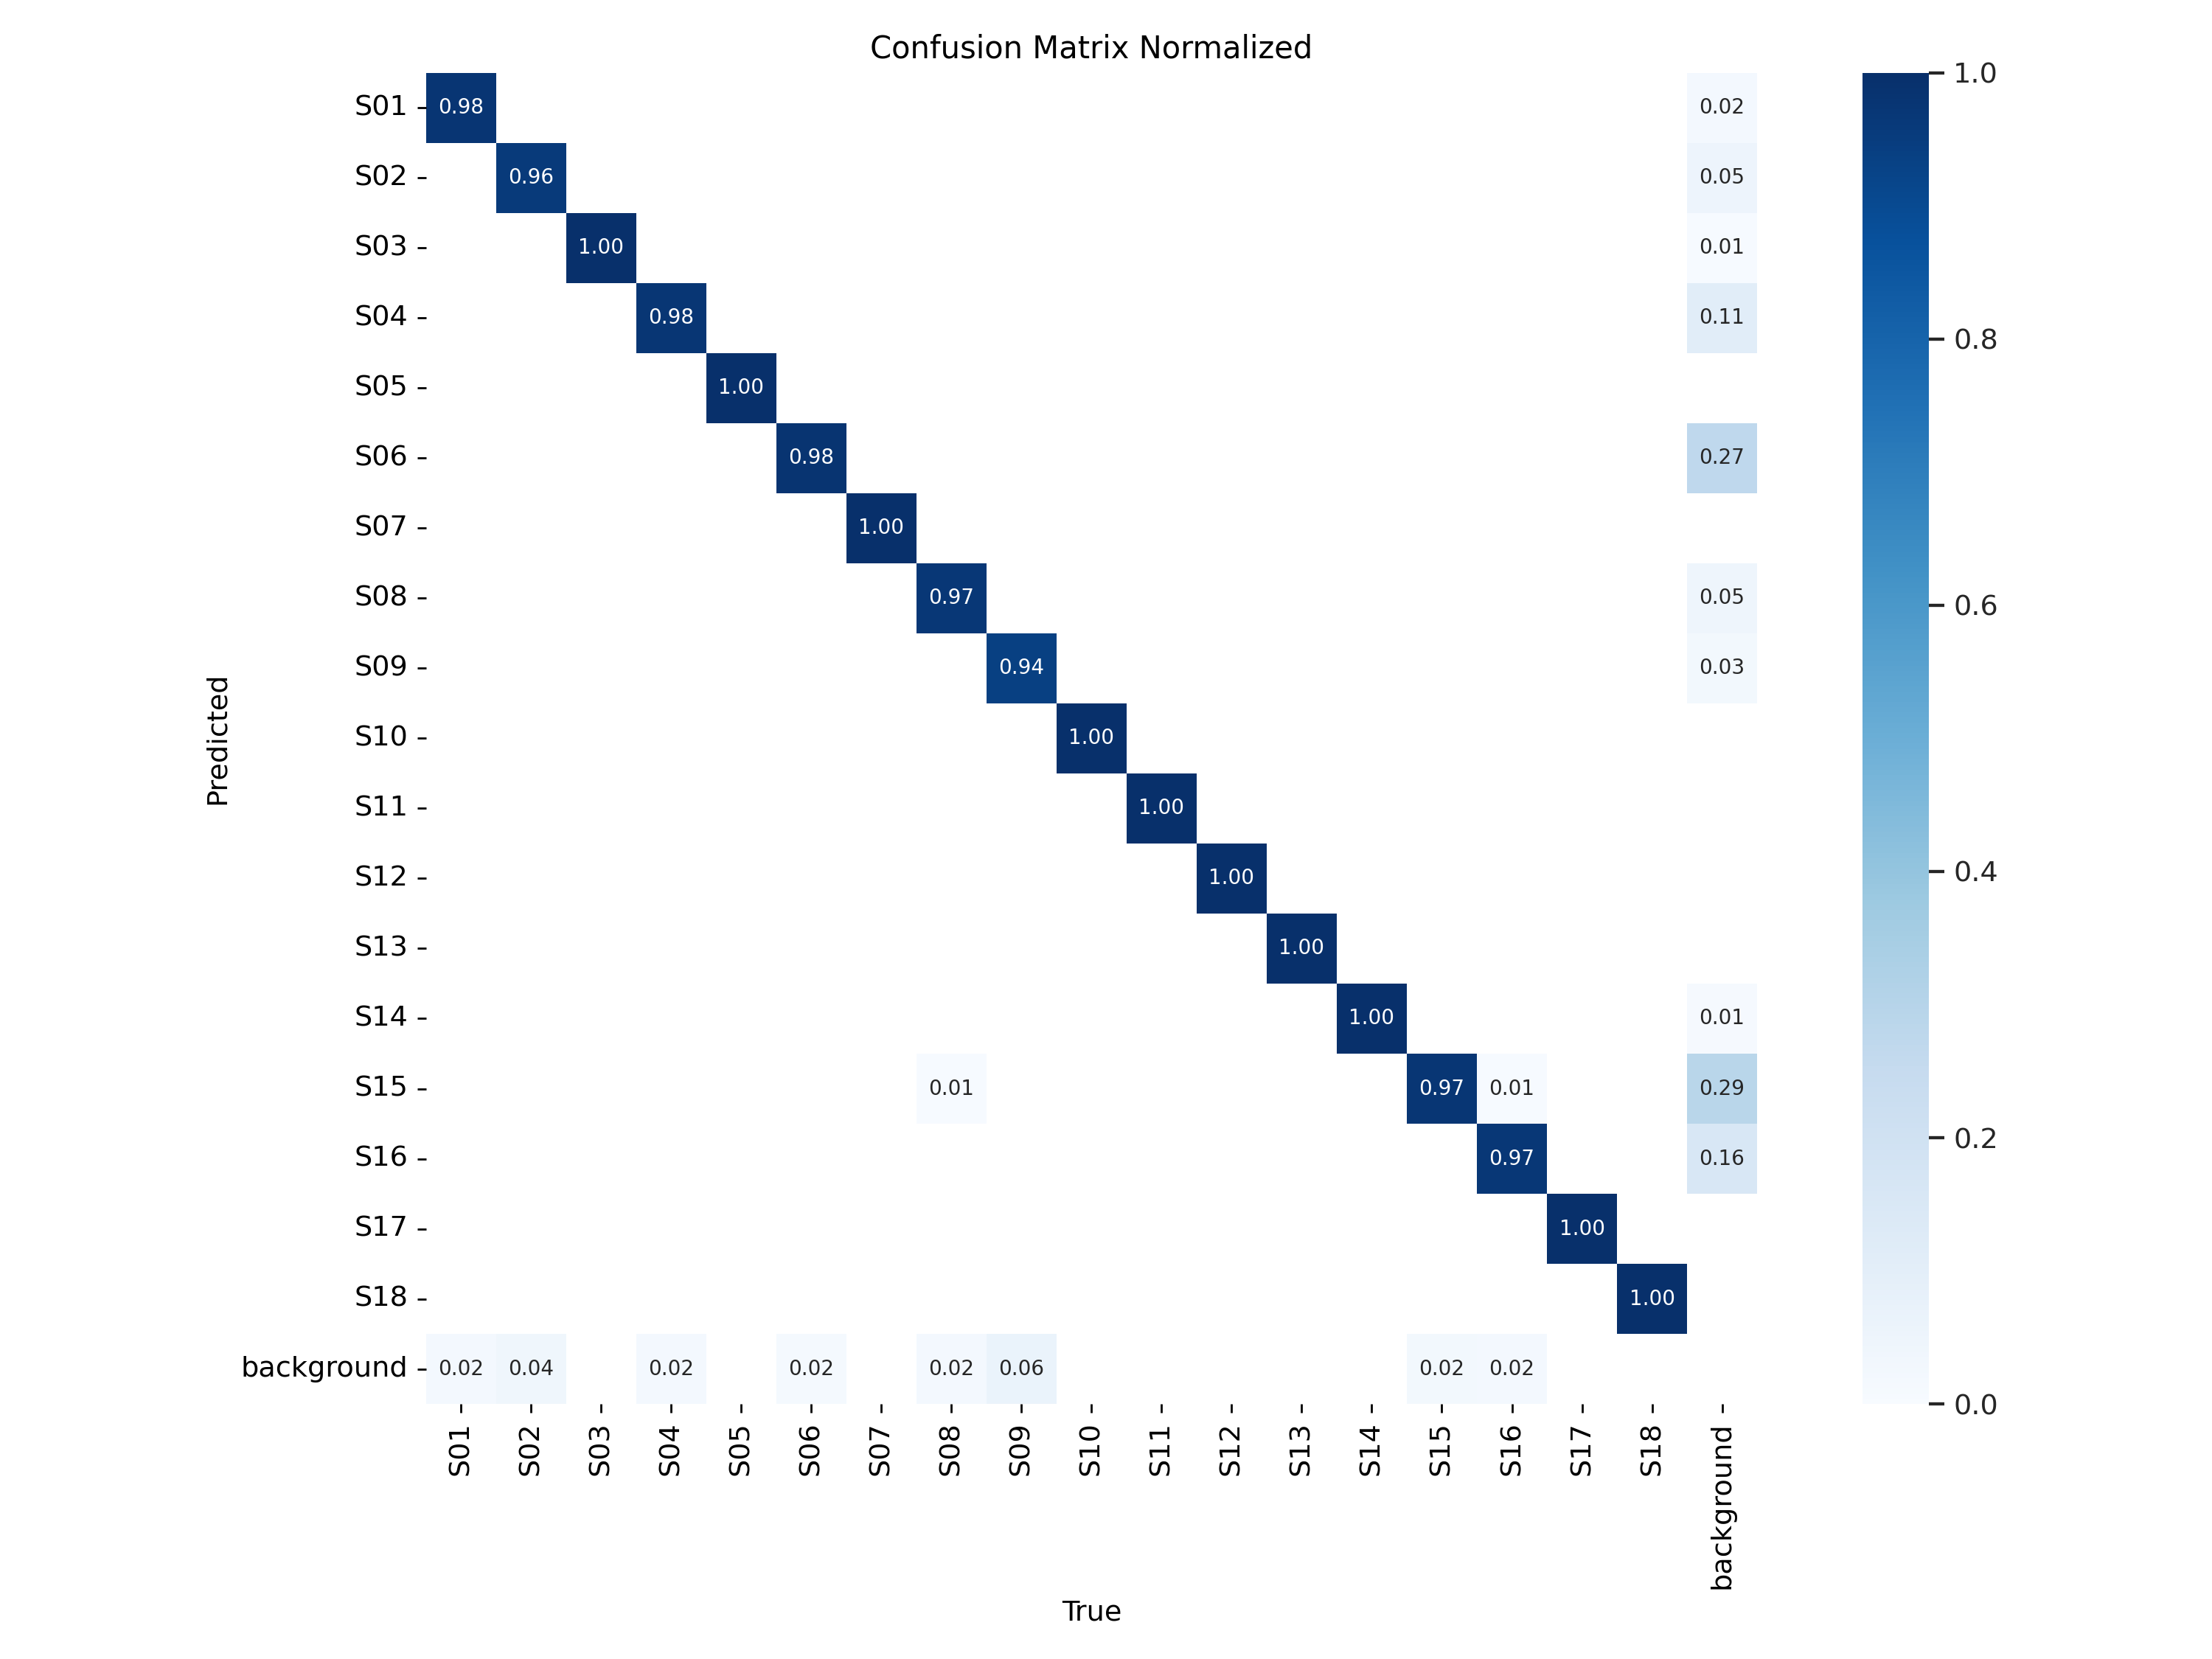
\includegraphics[width=0.85\textwidth]{figs/chap04/m_confusion_matrix_normalized.png}
    \caption{YOLOv11m混淆矩阵}
    \label{fig:mmatrix}
\end{figure}

\subsection{驾驶员id模型}
本文基于YOLOv11n、YOLOv11s和YOLOv11m三个模型,各训练了300个epoch,驾驶员id模型训练结果如\ref{fig:trackResult}所示。下面同样对七个检测精度指标进行详细对比分析。

\begin{figure}[H]
    \centering
    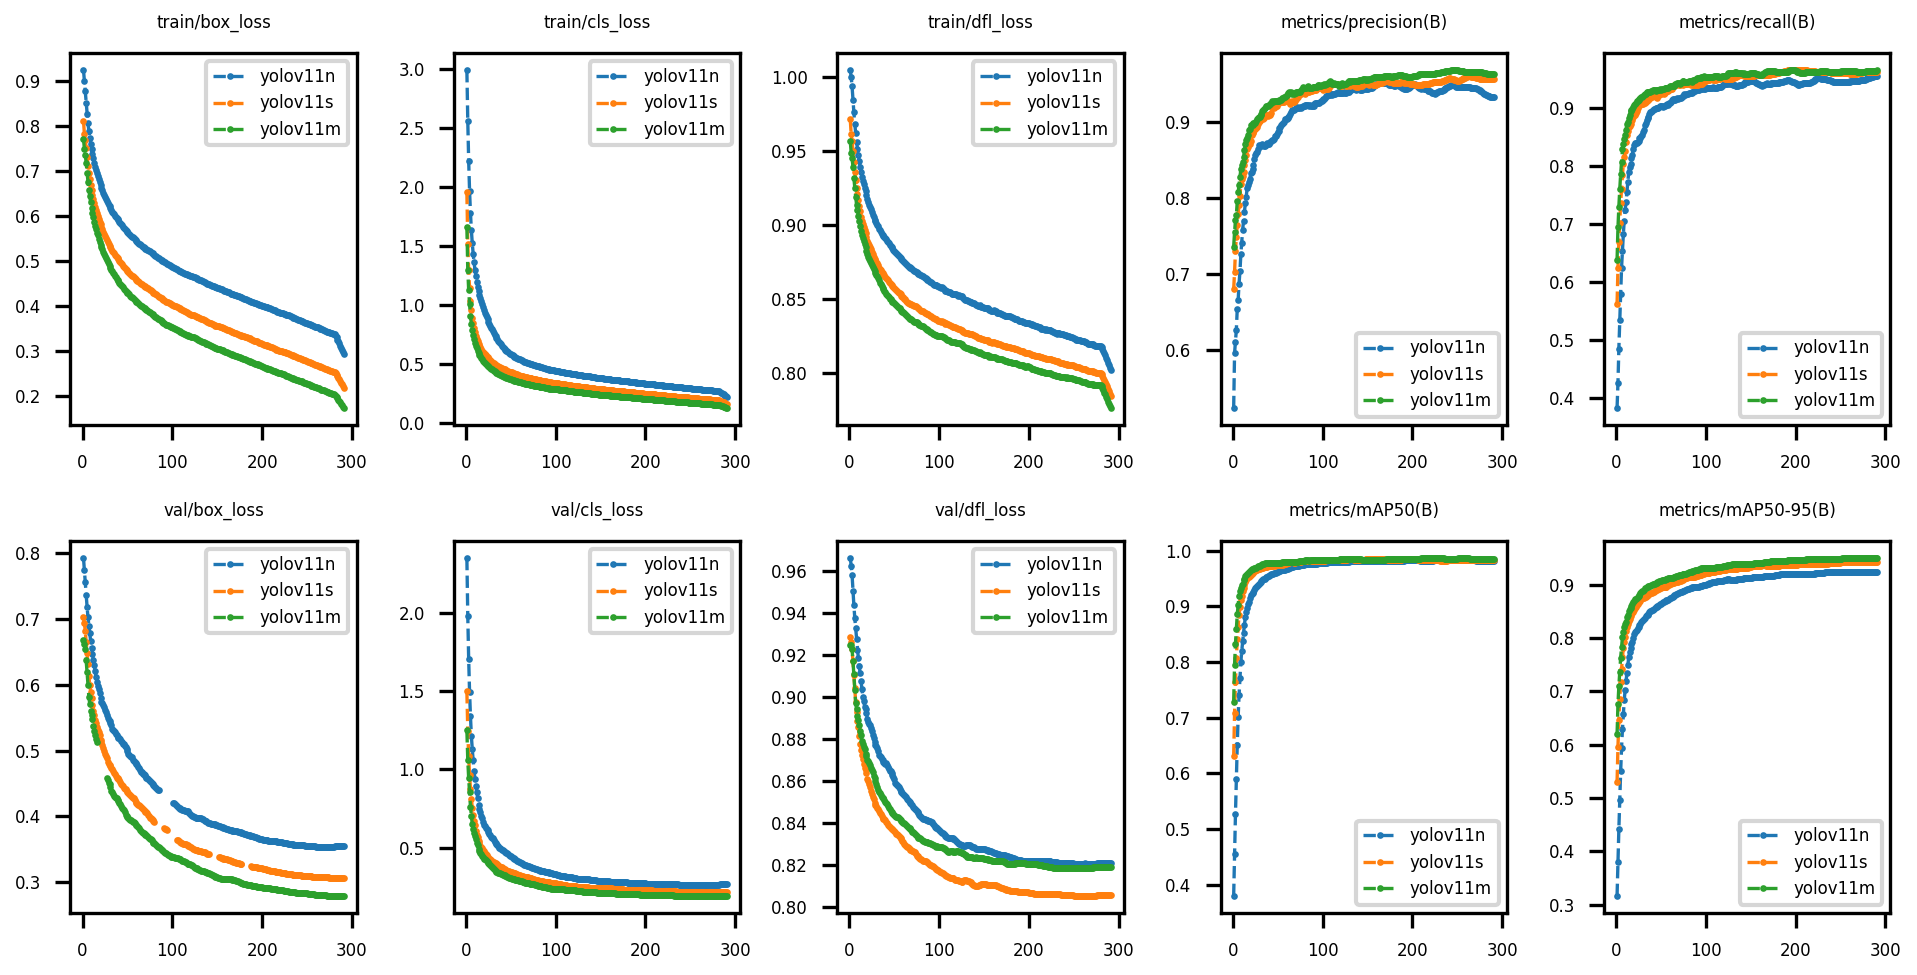
\includegraphics[width=1\textwidth]{figs/chap04/trackResult.png}
    \caption{驾驶员id模型}
    \label{fig:trackResult}
\end{figure}

边界框回归损失:YOLOv11s和YOLOv11m两个模型的边界框回归损失在前期下降速度相较于YOLOv11n略快,中期以后三者下降速度相近。YOLOv11m训练得到的边界框回归损失最优,数值最小,YOLOv11s次之,YOLOv11n相对较高。说明YOLOv11m模型预测驾驶员id的边界框更精确。

分类损失:YOLOv11s和YOLOv11m的分类损失在前期下降较快,YOLOv11n稍慢一些,中期以后三者下降速度近似。YOLOv11m的分类损失值最小,其次是YOLOv11s,YOLOv11n的值最高。YOLOv11m模型对驾驶员id的分类效果更好。

分布损失:YOLOv11m和YOLOv11s的分类损失值收敛较快,YOLOv11n收敛相对较慢。训练结束时YOLOv11m的分布损失值最小,效果最好,YOLOv11s次之,YOLOv11n的值最大。

精度:YOLOv11m收敛速度最快,最早到达较高水平并趋于平稳。YOLOv11n和YOLOv11s上升速度相对较慢。最终YOLOv11m的精度最高,其次是YOLOv11s,YOLOv11n的精度最低。这表明YOLOv11m对驾驶员id的预测更准确。

召回率:YOLOv11m和YOLOv11s的收敛趋势近似,且都比YOLOv11n的收敛速度要快。YOLOv11m和YOLOv11s最终的召回率相近,都比YOLOv11n的召回率要高。说明YOLOv11m和YOLOv11n能找到更多的正例驾驶员id目标。

mAP50:YOLOv11m和YOLOv11s的mAP50值收敛趋势比较相似,都比YOLOv11n的收敛速度要快。最终三个模型的mAP50值几乎相同。

mAP50-95:YOLOv11m的mAP50-95值收敛速度最快,其次是YOLOv11s,YOLOv11n的收敛速度最慢。训练结束时,YOLOv11m的mAP50-95最高,效果最优;YOLOv11s次之;YOLOv11n相对较低。

将上述七个指标训练过程中的最优值进行对比如\ref{tab:modelCompare2}。三个损失函数(box\_loss、cls\_loss、dfl\_loss)随模型规模增大,最优值不断减小;四个精度指标(precision、recall、mAP50、mAP50-95)则随模型规模增大,最优值持续升高,模型检测精度随之提升。

\begin{table}[htb]
    \centering
    \caption[指标对比]{模型损失函数与检测精度指标对比2\label{tab:modelCompare2}}
    \begin{tabular}{lccccccc}
        \toprule
        Model & 
        \makecell{box\_loss\\(\%)} & 
        \makecell{cls\_loss\\(\%)} & 
        \makecell{dfl\_loss\\(\%)} & 
        \makecell{Precision\\(\%)} & 
        \makecell{Recall\\(\%)} & 
        \makecell{mAP50\\(\%)} & 
        \makecell{mAP50-95\\(\%)} \\
        \midrule
        YOLOv11n & 28.5 & 21.9 & 79.9 & 95.6 & 95.8 & 98.3 & 92.5 \\
        YOLOv11s & 21.0 & 15.7 & 78.2 & 96.1 & 96.7 & 98.7 & 94.3 \\
        YOLOv11m & 16.6 & 12.4 & 77.3 & 96.9 & 96.9 & 98.7 & 95.0 \\
        \bottomrule
    \end{tabular}
\end{table}

三个模型的检测速度对比如\ref{tab:speedCompare2}。随着模型规模增大,每秒处理帧数降低,实时性变差;且FLOPs数值增大,说明在预测中进行的浮点运算次数更多,理论上需要更长的推理时间。

\begin{table}[htb]
    \centering
    \caption[目标数据]{模型检测速度对比2\label{tab:speedCompare2}}
    \begin{tabular}{lcc}
        \toprule
        Model & 
        \makecell{FPS(1)} & 
        \makecell{FLOPs(G)} \\
        \midrule
        YOLOv11n & 67.11 & 7.49 \\
        YOLOv11s & 66.67 & 22.68 \\
        YOLOv11m & 55.87 & 70.45 \\
        \bottomrule
    \end{tabular}
\end{table}

% \subsection{YOLOv11n}
% 本文基于YOLOv11n训练了300个epoch,训练结果如\ref{fig:nresult}所示。从实验结果可知,模型的最高精度为96.7\%,最高召回率为96.6\%,mAP50为99.0\%,mAP50-95为94.1\%。
% \begin{figure}[H]
%     \centering
%     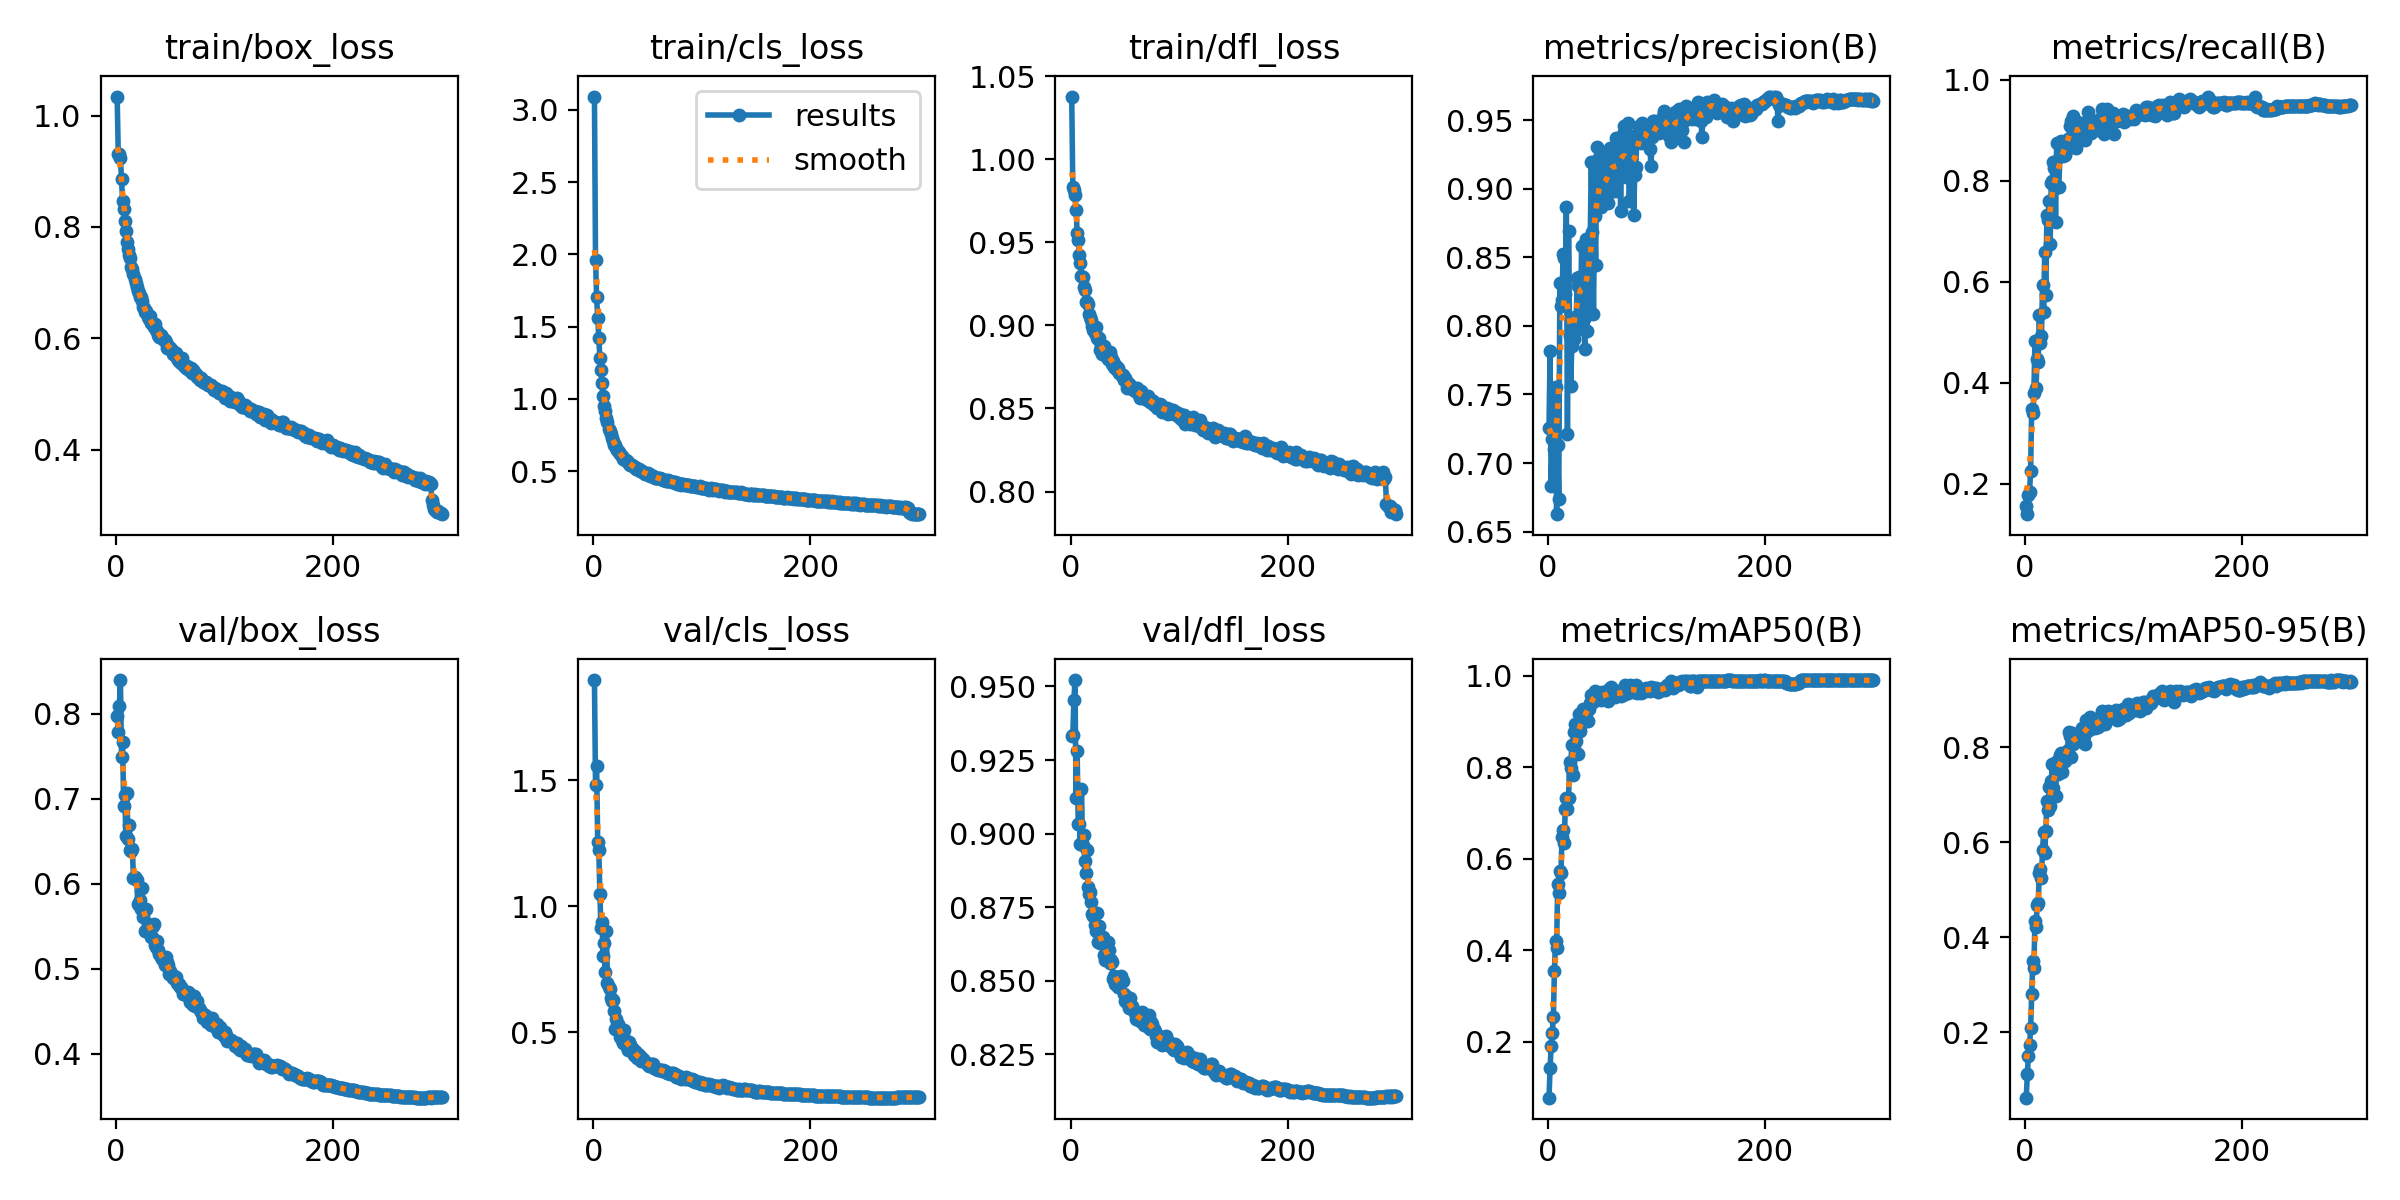
\includegraphics[width=0.8\textwidth]{figs/chap04/n_results.png}
%     \caption{YOLOv11n训练结果}
%     \label{fig:nresult}
% \end{figure}

% 基于YOLOv11n训练出的模型的混淆矩阵见\ref{fig:nmatrix},模型对大部分目标的分类效果都不错,18个标签中有15个标签的判断准确率达到了97\%。对S07这一类别的分类效果较差,对其中33\%的数据都预测为了S10,仅有67\%的正确率。该模型的P-R曲线见\ref{fig:npr},可以看出mAP@0.5为99.0\%。



% \begin{figure}[H]
%     \centering
%     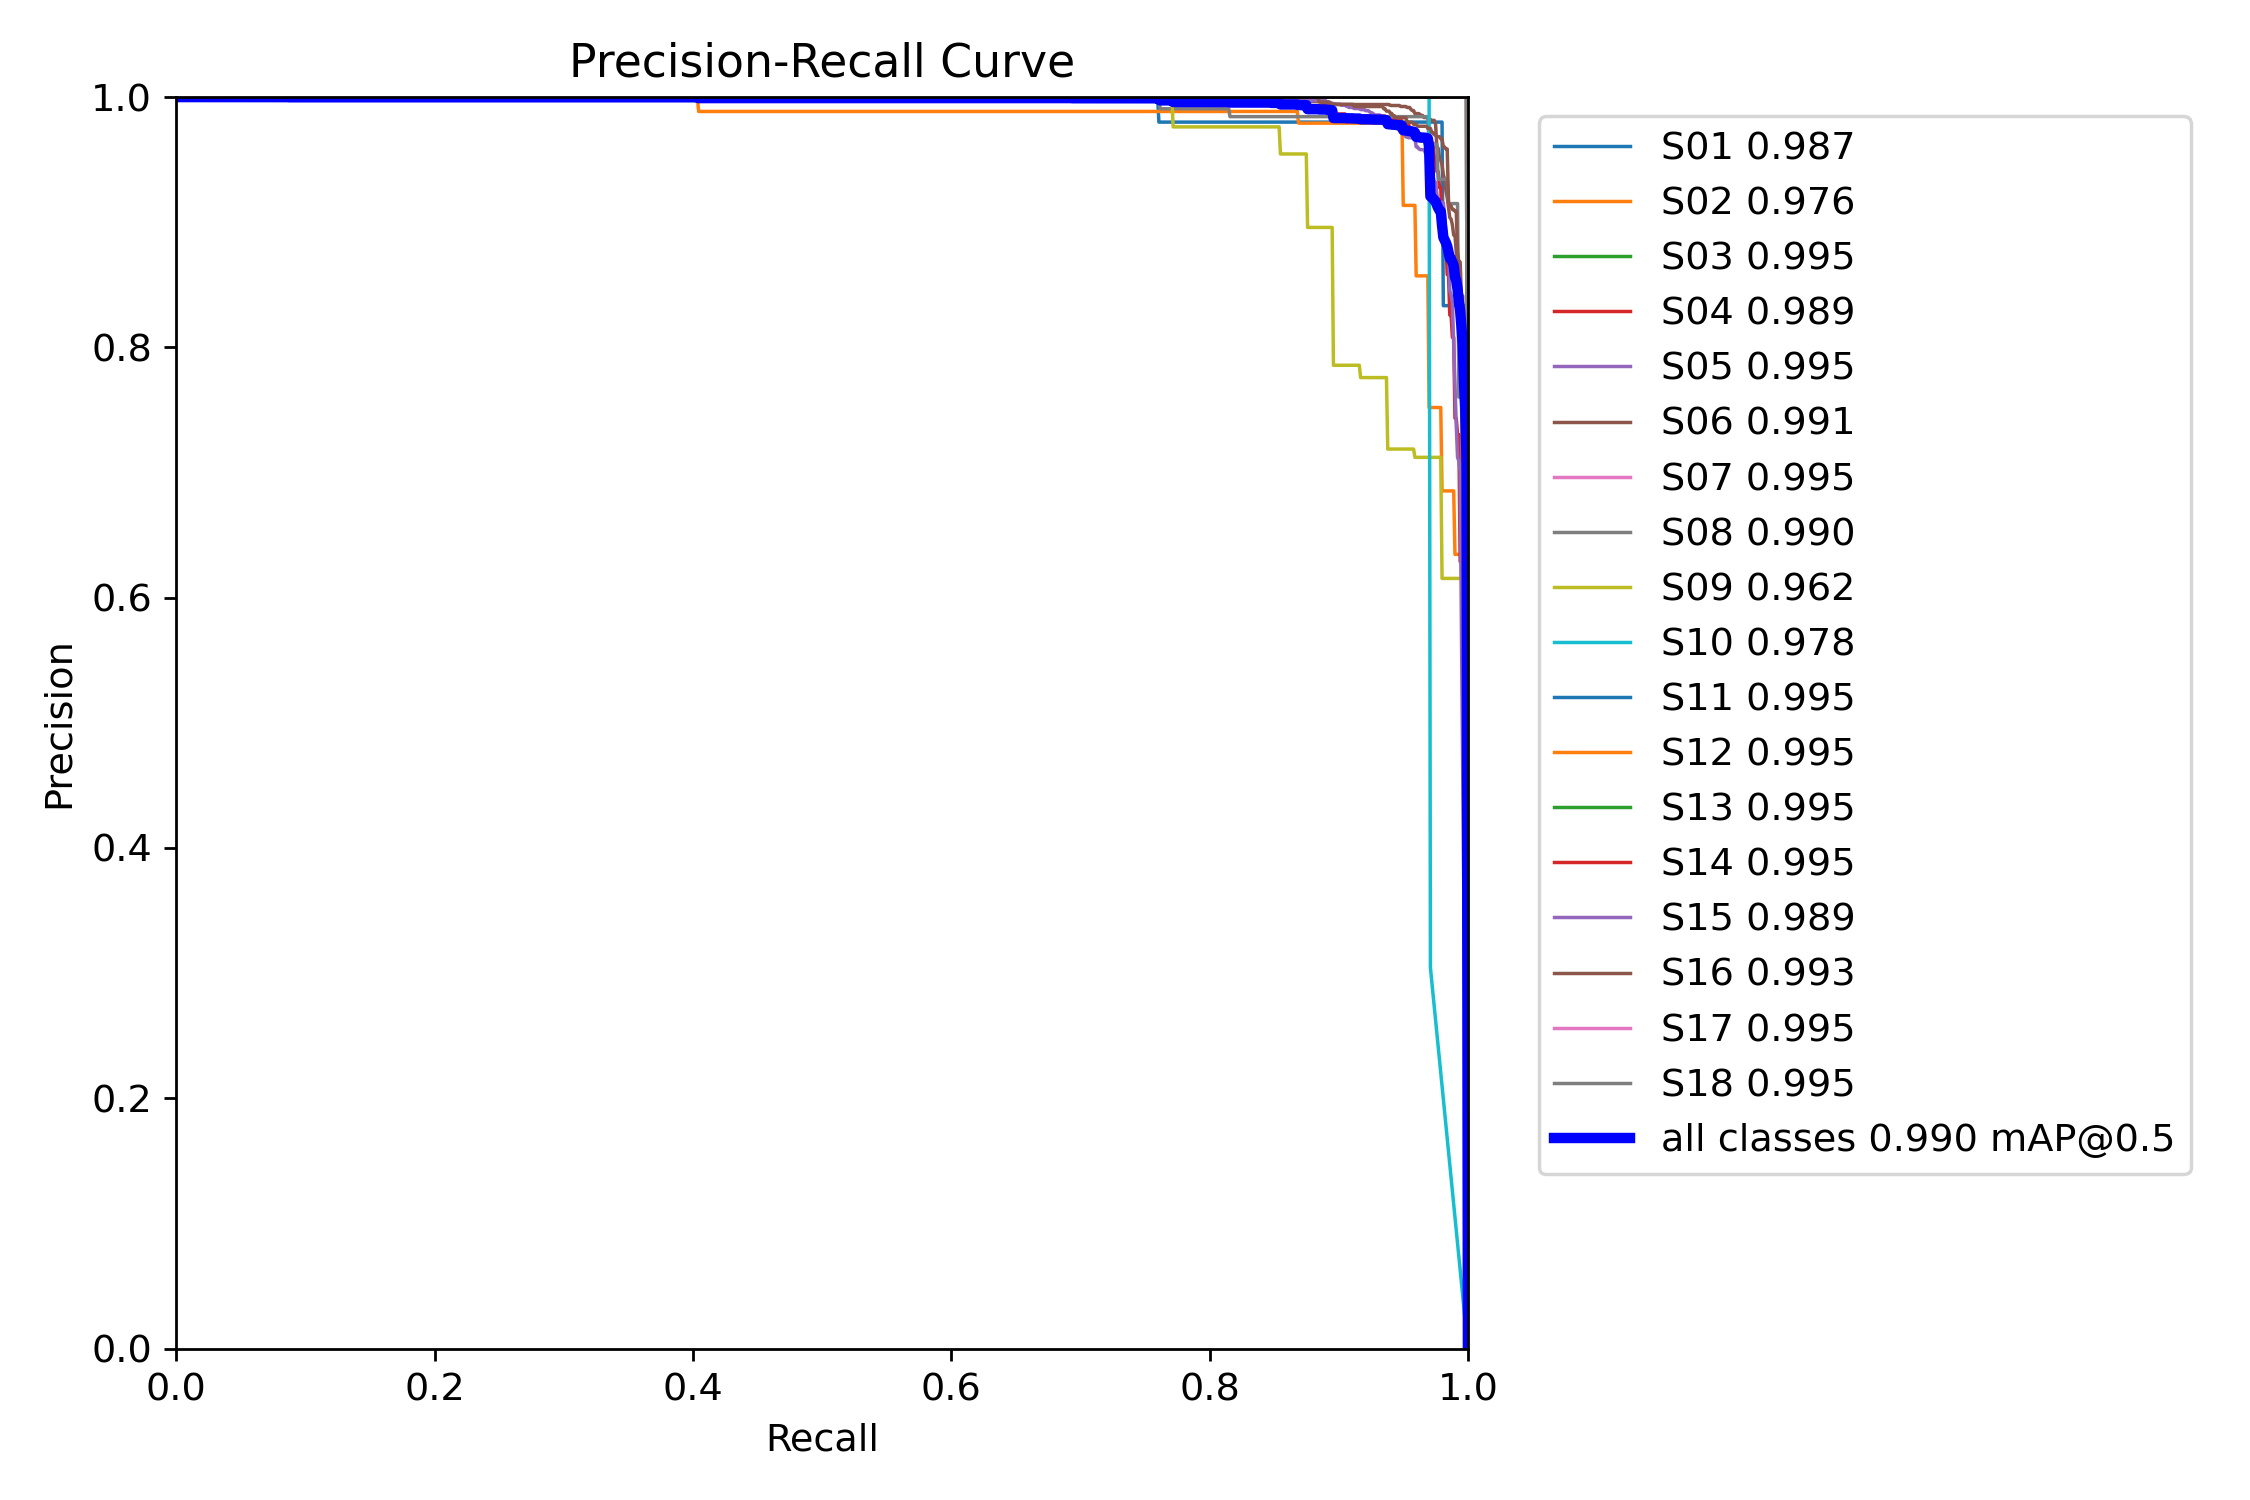
\includegraphics[width=0.6\textwidth]{figs/chap04/n_PR_curve.png}
%     \caption{YOLOv11nP-R曲线}
%     \label{fig:npr}
% \end{figure}

% \subsection{YOLOv11s}
% 本文基于YOLOv11s训练了300个epoch,训练结果见\ref{fig:sresult}。该模型的最高精度为96.2\%,最高召回率为97.2\%,mAP50为99.0\%,mAP50-95为95.4\%。

% \begin{figure}[H]
%     \centering
%     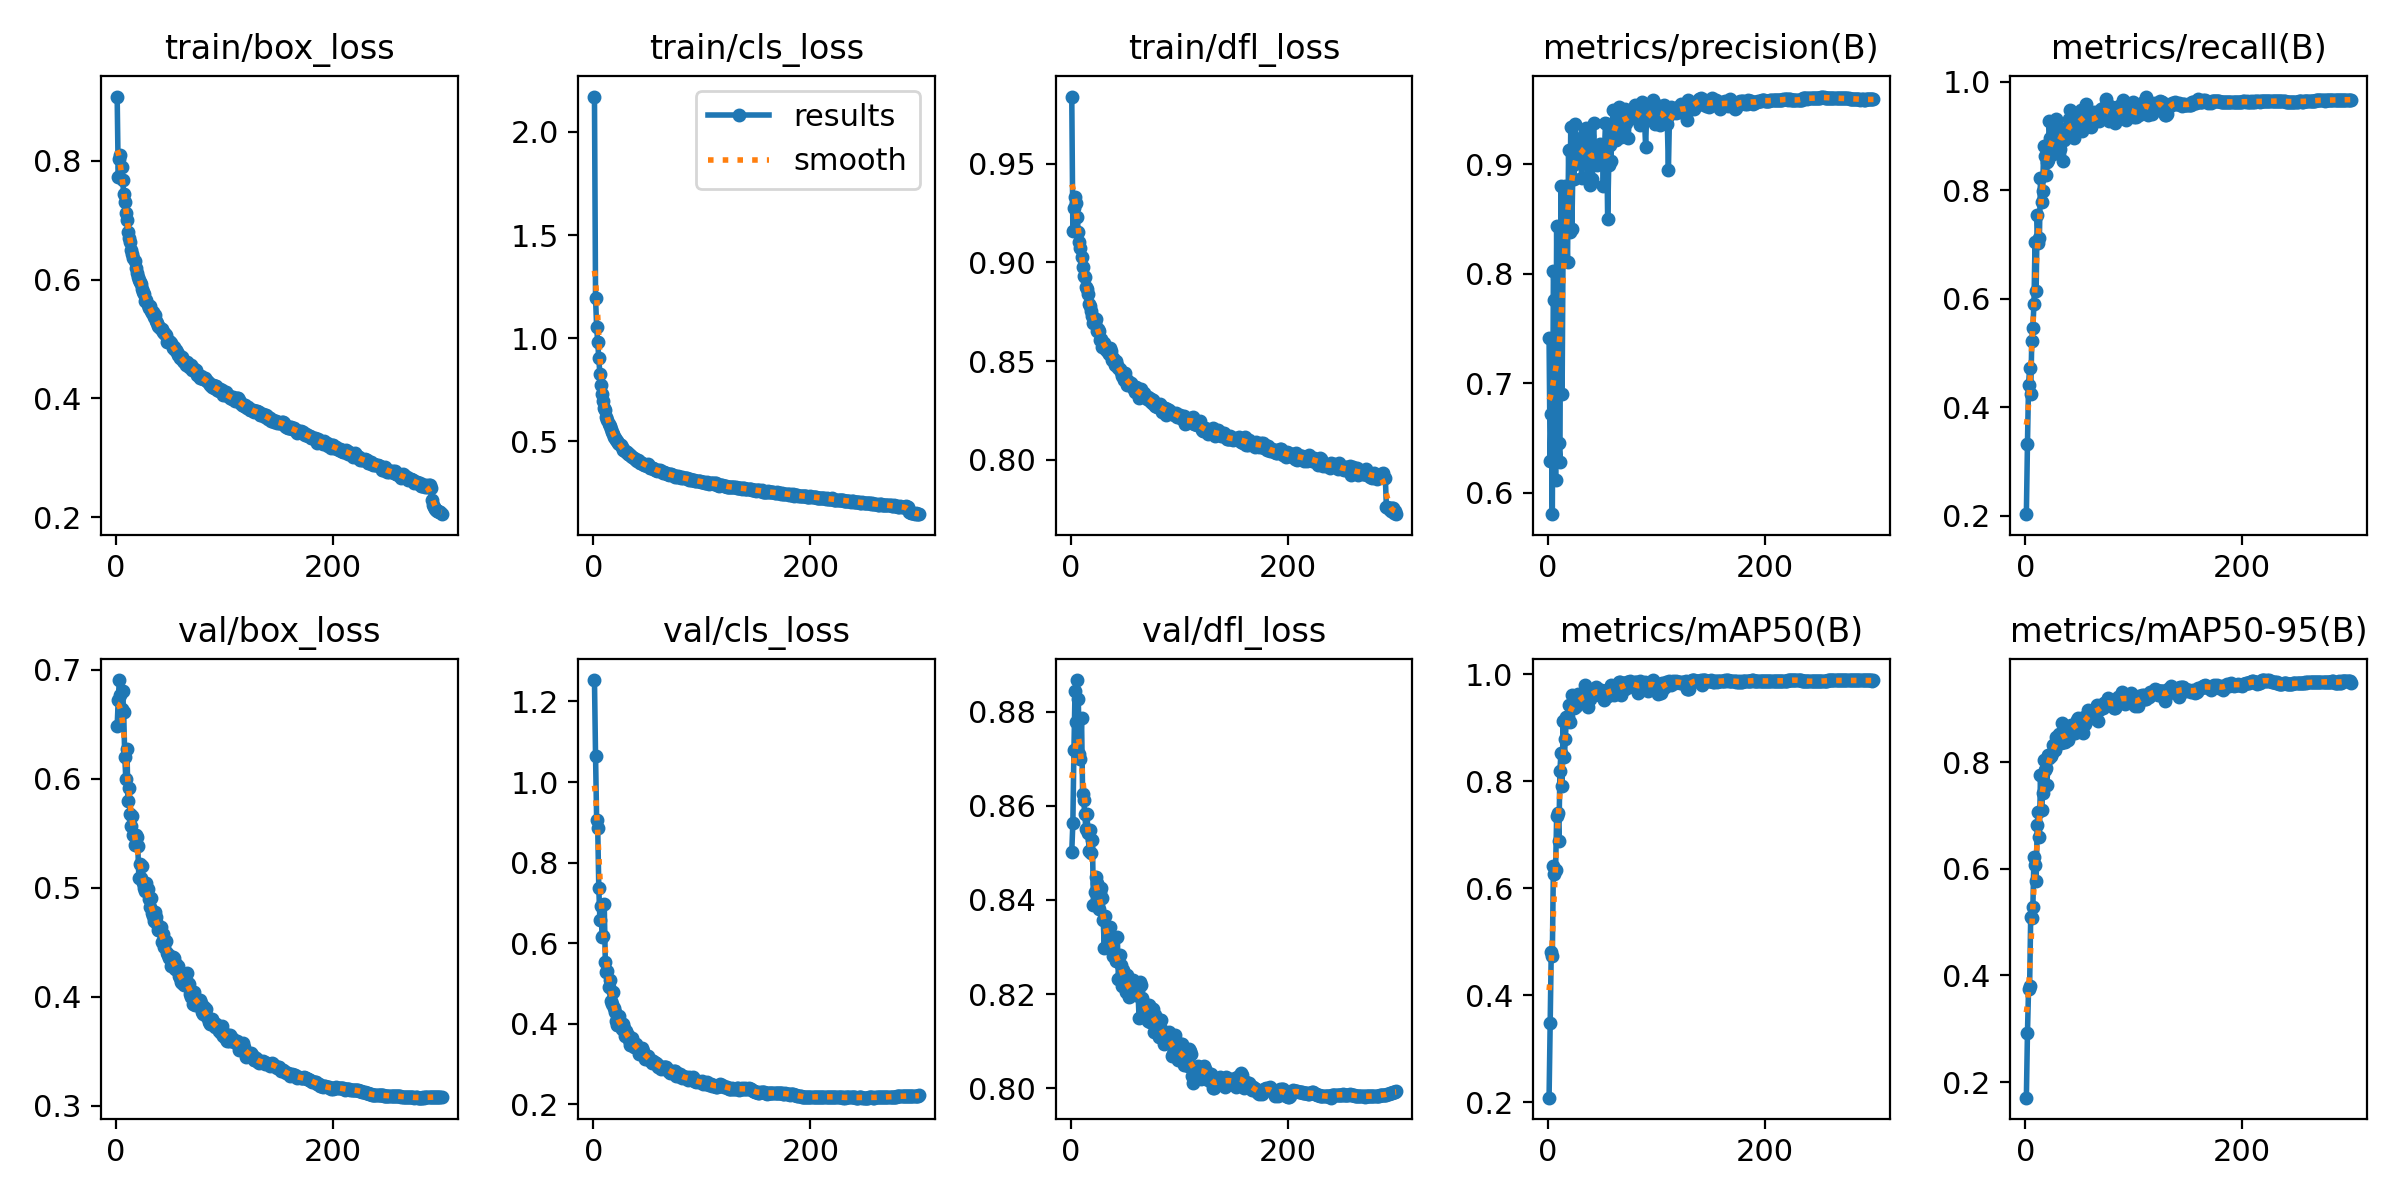
\includegraphics[width=0.8\textwidth]{figs/chap04/s_results.png}
%     \caption{YOLOv11s训练结果}
%     \label{fig:sresult}
% \end{figure}

% \ref{fig:smatrix}展示了该模型的混淆矩阵,可以看出模型对S01类别有6\%的误判,其中2\%预测为了S04,4\%预测为了S06。对S09类别有2\%的误判,预测成了S06,以及4\%的漏判,其他的类别的准确率都达到了97\%。YOLOv11s训练结果的P-R曲线如\ref{fig:spr},该模型的mAP@0.5为99.0\%。




% \begin{figure}[H]
%     \centering
%     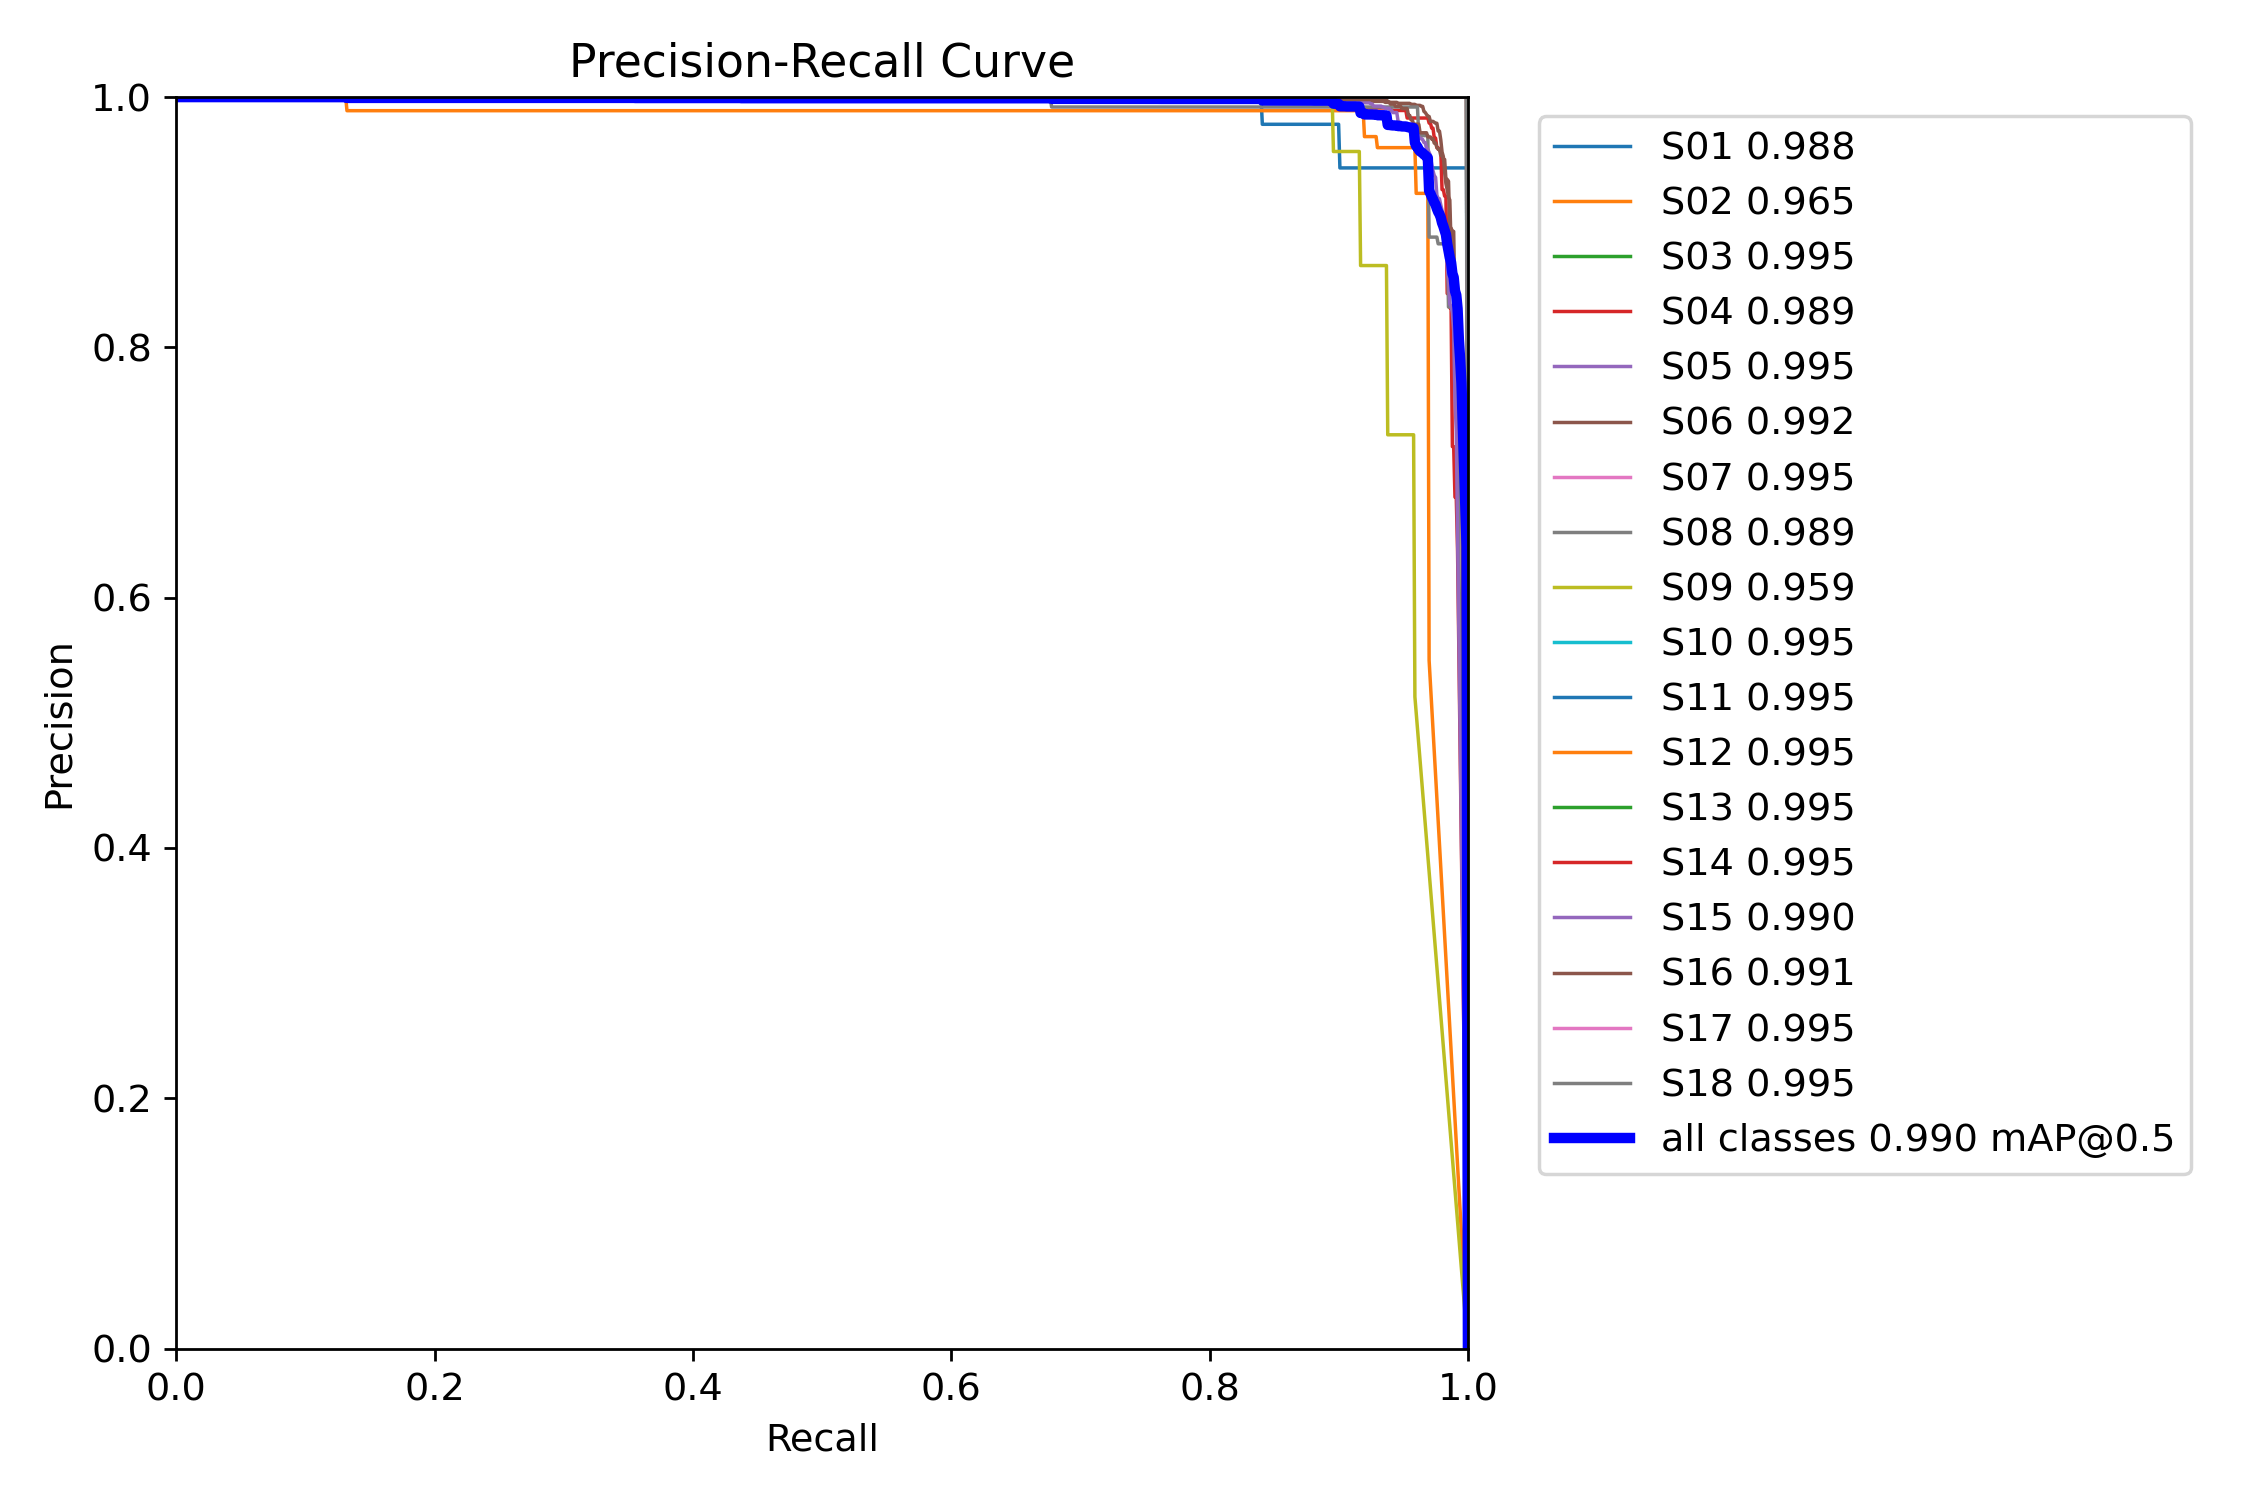
\includegraphics[width=0.6\textwidth]{figs/chap04/s_PR_curve.png}
%     \caption{YOLOv11sP-R曲线}
%     \label{fig:spr}
% \end{figure}

% \subsection{YOLOv11m}
% 本文基于YOLOv11m训练了300个epoch,实验结果如\ref{fig:mresult}所示,该模型的最高精度为97.3\%,最高召回率为98.1\%,mAP50为99.1\%,mAP50-95为95.5\%。

% \begin{figure}[H]
%     \centering
%     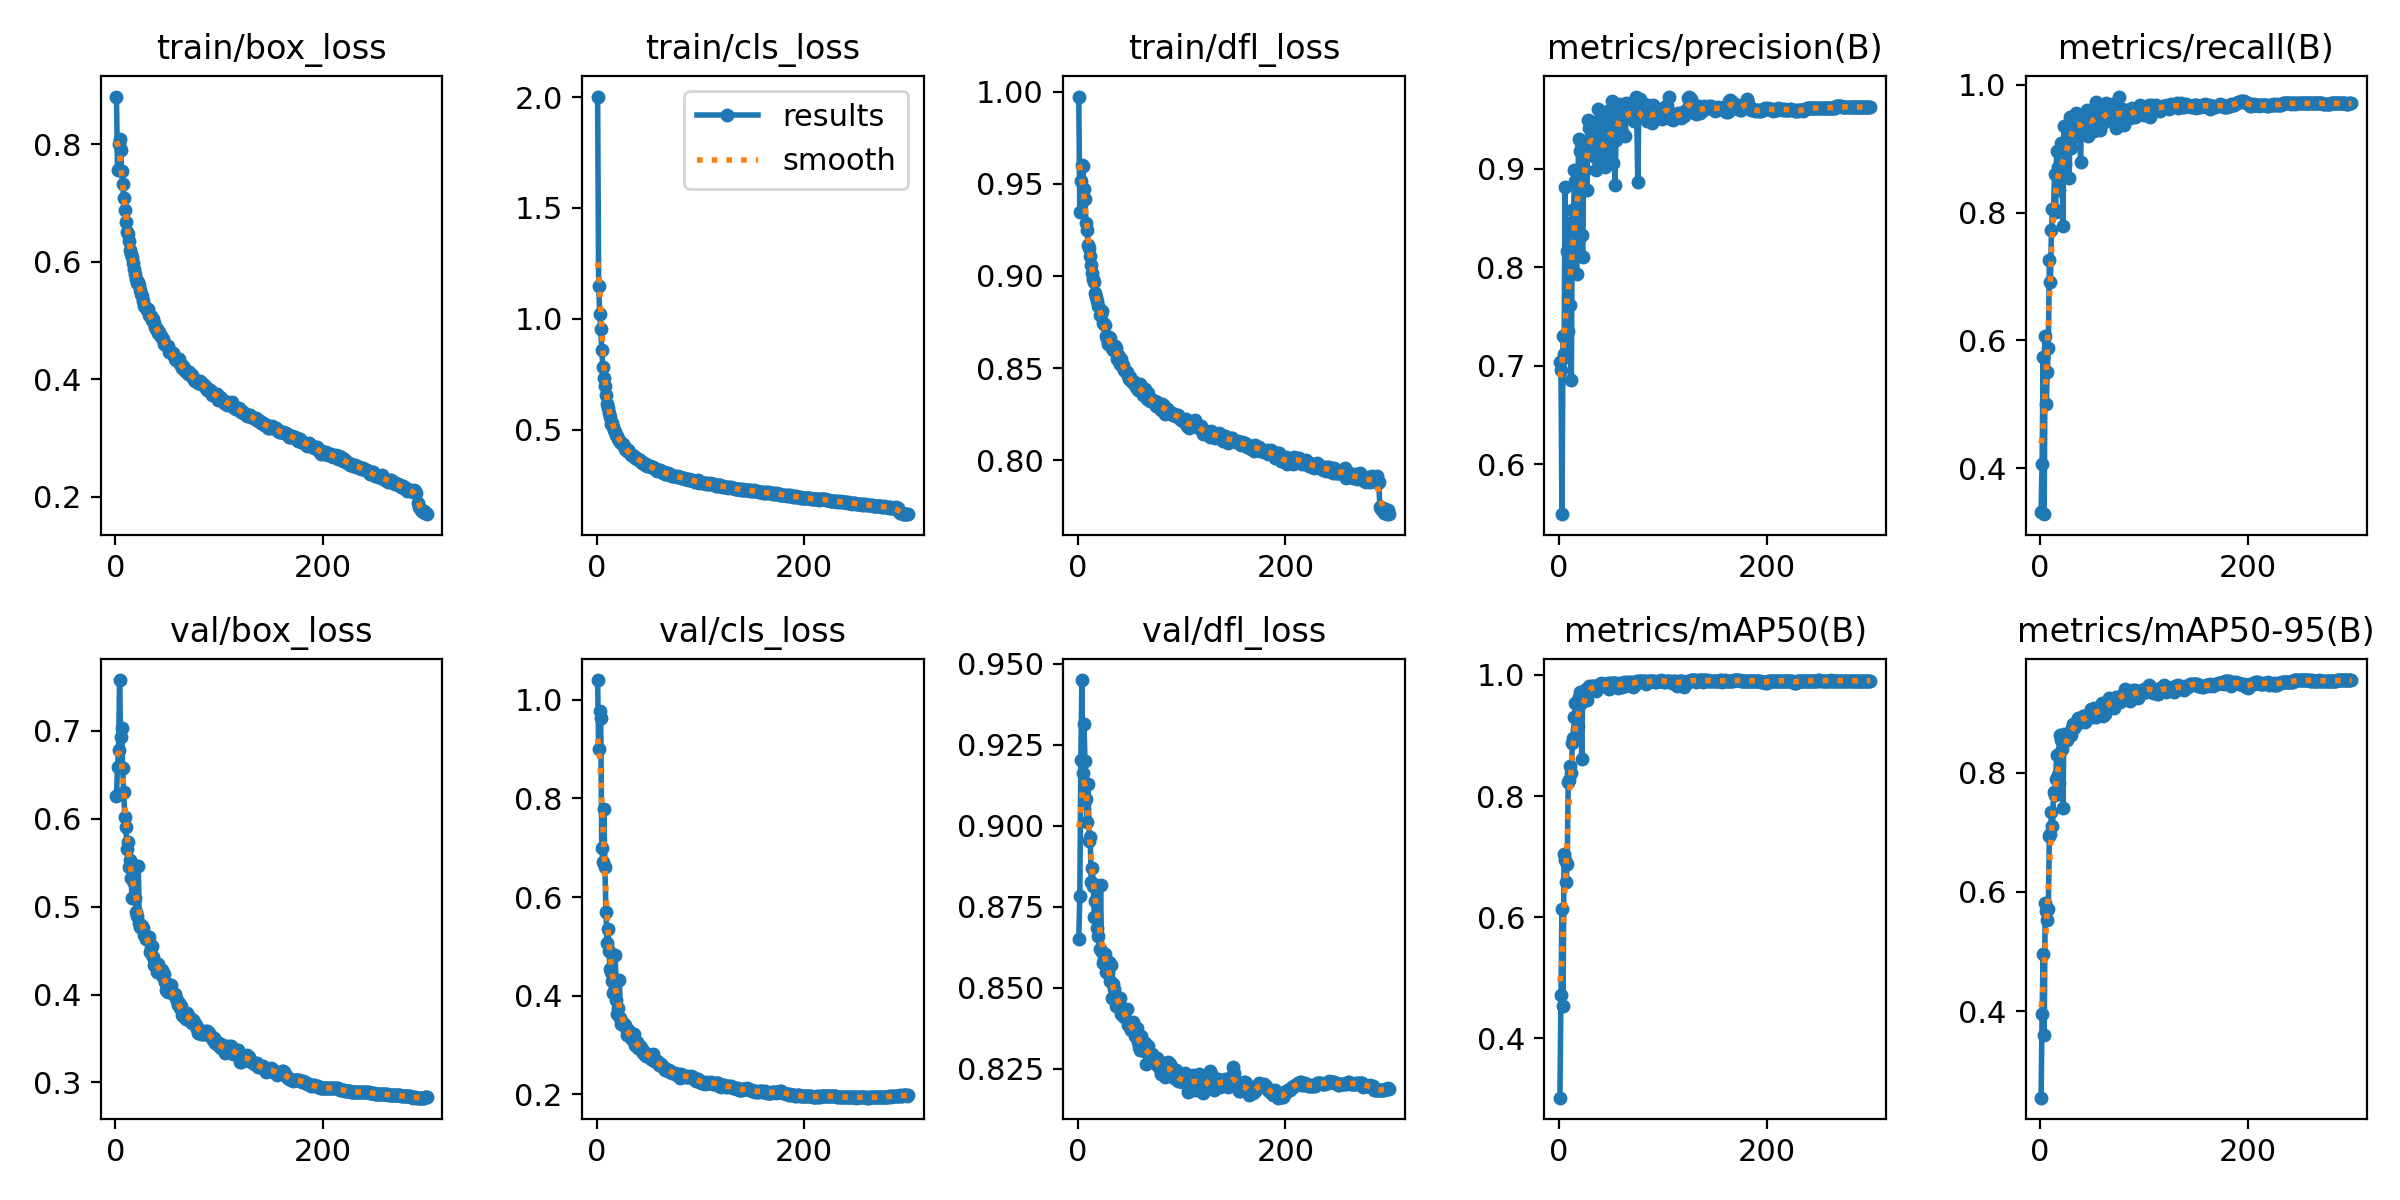
\includegraphics[width=0.8\textwidth]{figs/chap04/m_results.png}
%     \caption{YOLOv11m训练结果}
%     \label{fig:mresult}
% \end{figure}

% 混淆矩阵如\ref{fig:mmatrix}所示,模型对S04类别有4\%的漏判,对S9类别有6\%的漏判,其他类别的准确率都达到了97\%。P-R曲线为\ref{fig:mpr},该模型的mAP@0.5为99.1\%。

% \begin{figure}[H]
%     \centering
%     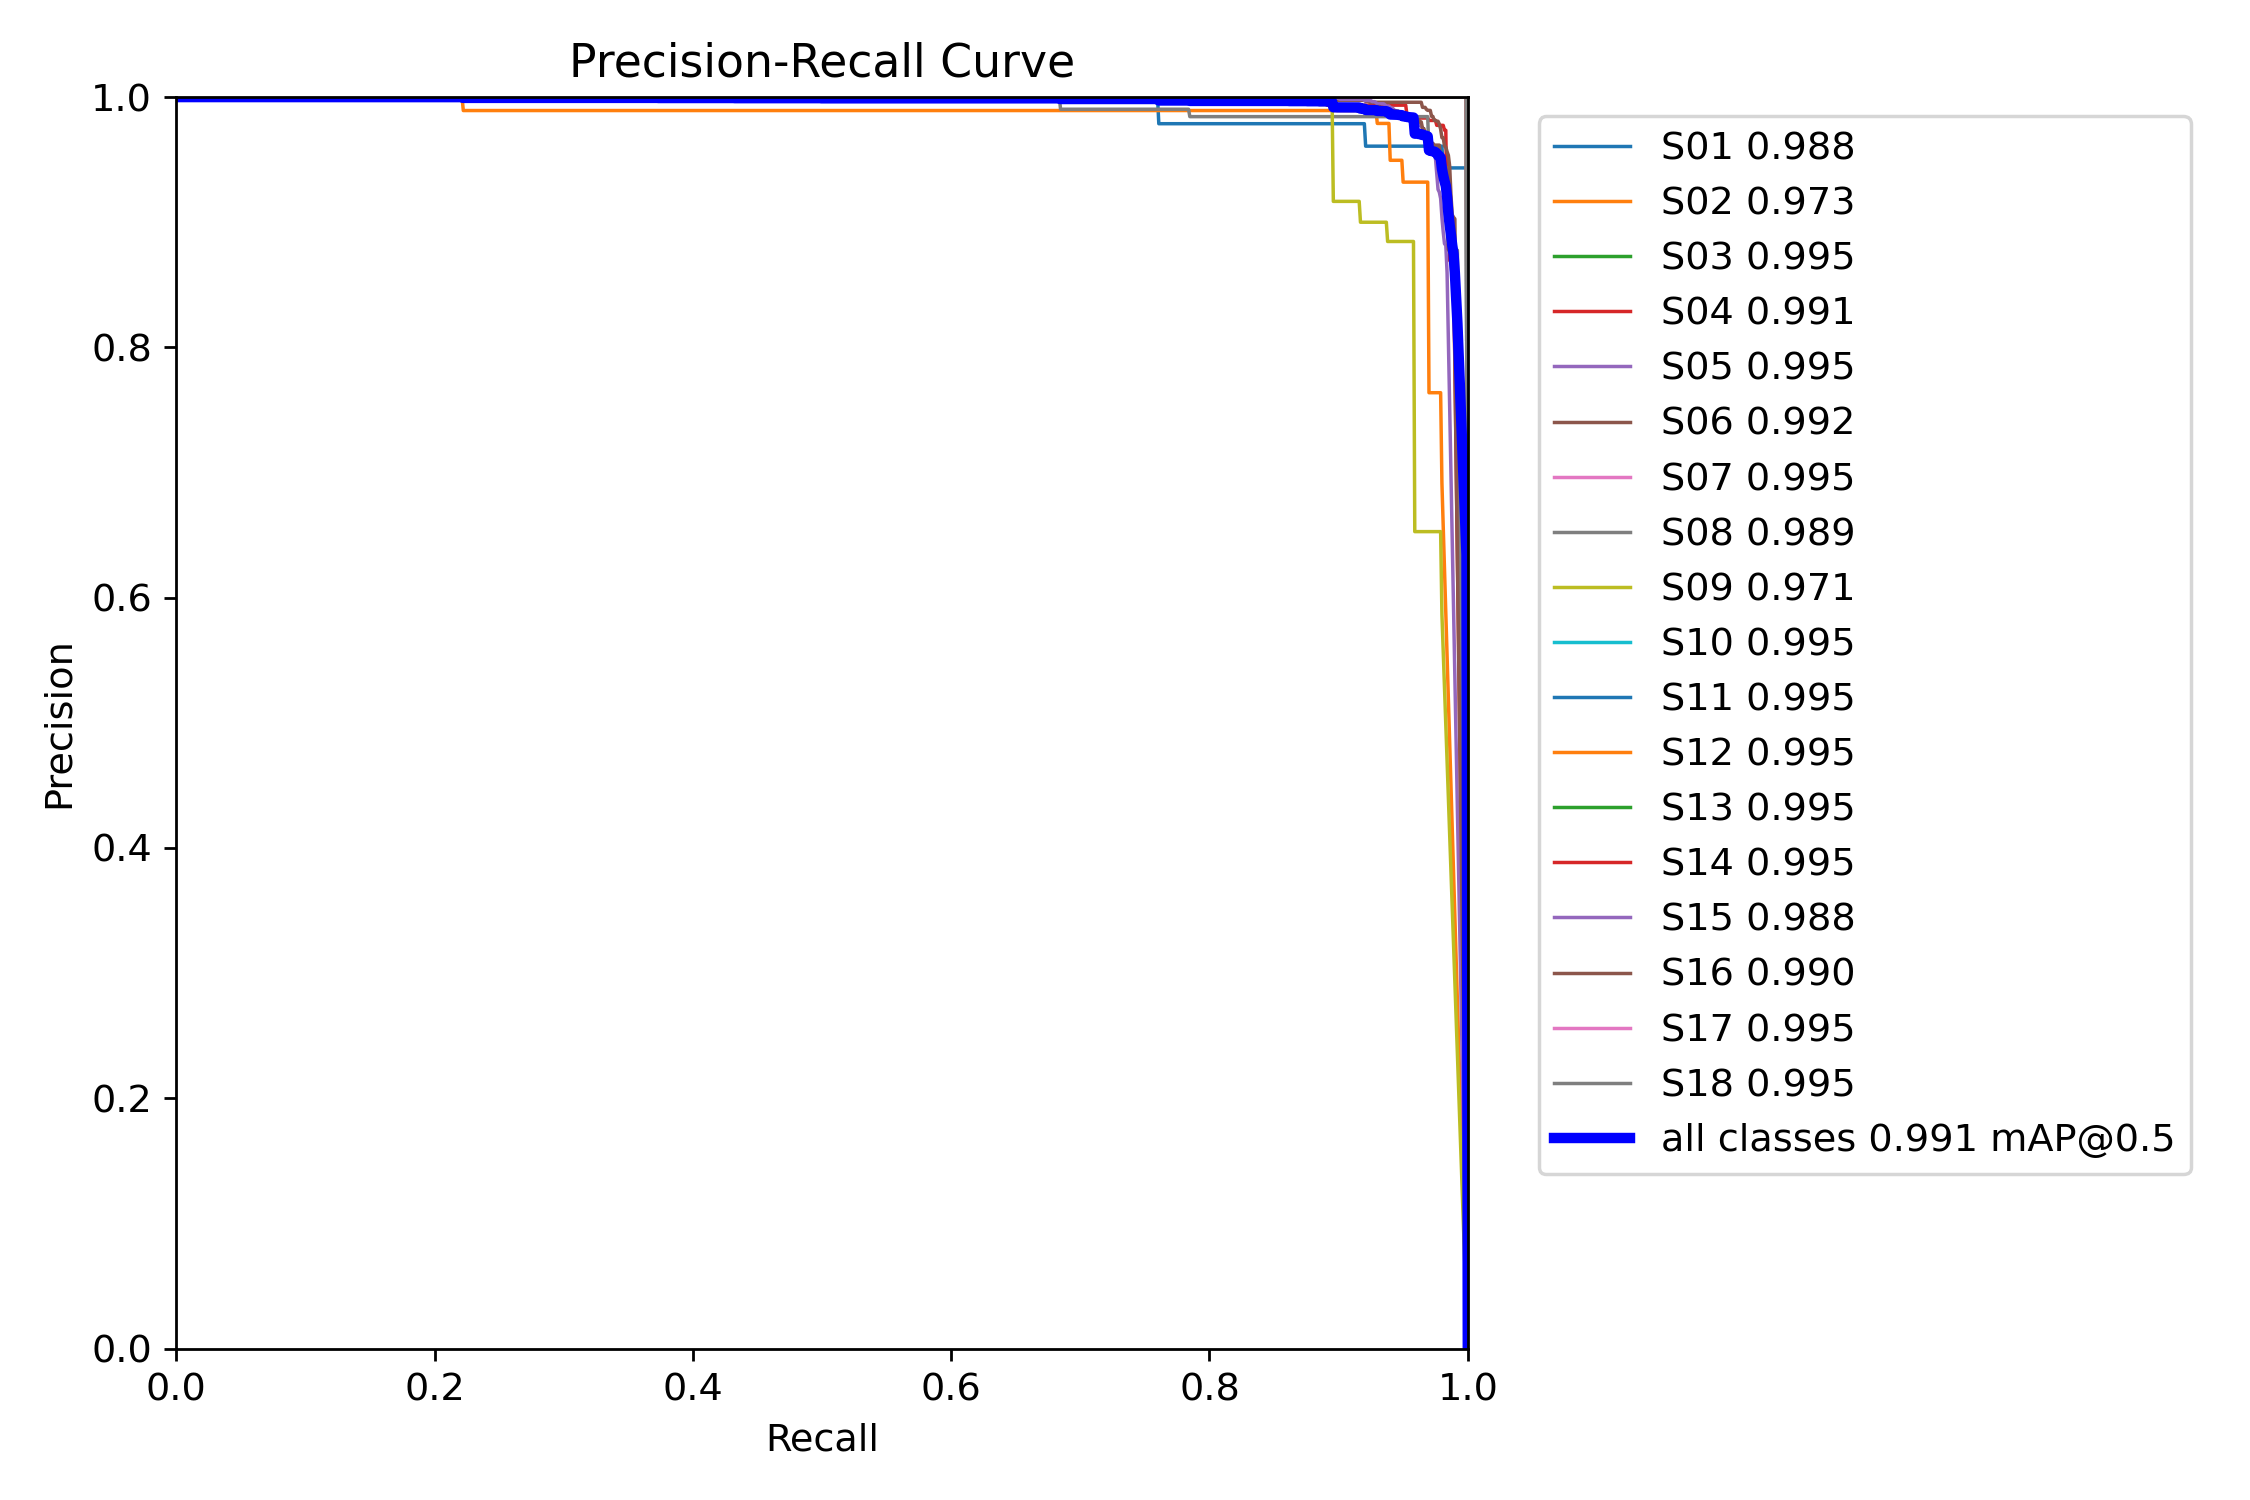
\includegraphics[width=0.6\textwidth]{figs/chap04/m_PR_curve.png}
%     \caption{YOLOv11mP-R曲线}
%     \label{fig:mpr}
% \end{figure}

% \subsection{模型性能对比}
% 本文基于YOLOv11三种不同的模型对摩托车驾乘人员头盔佩戴数据集进行了训练,\ref{tab:modelCompare}展示了各个模型在精度、召回率、mAP50、mAP50-95以及检测速度这五个方面的对比。

% 三个模型的精度均在96\% 以上。其中,YOLOv11m的精度最高,为97.3\%。三个模型的召回率也都处于较高水平,都在96\%以上。YOLOv11m的召回率最高,为98.1\%。三个模型的mAP50值几乎一致,都在99\%附近,最大仅相差0.1\%,说明在IoU阈值为0.5时,它们对目标物体的检测效果都非常好。在mAP50-95指标上,YOLOv11m和YOLOv11s表现较好,分别为95.5\%和95.4\%,仅相差0.1\%,都要高于YOLOv11n的94.1\%,这表明在更严格的IoU阈值范围内,YOLOv11m和YOLOv11s 的性能更优。

% 在检测速度方面,平均检测一张图片YOLOv11m耗时最长,为31.5ms,YOLOv11s为27.3ms,比YOLOv11m快了13.3\%。YOLOv11n最快,为24ms,比YOLOv11s快了12.1\%,比YOLOv11m快了23.8\%。

% 根据分析可知,YOLOv11n在速度上具有明显优势,适用于对实时性要求较高的场景。YOLOv11s 在精度和速度之间取得了较好的平衡,属于一个适中的模型。YOLOv11m牺牲了一定的检测速度,换来了更高的精度,适合对检测精度要求极高的场景。


\section{本章小结}
本章首先介绍了目标检测模型检测精度和检测速度的几个重要评价指标,然后对本文进行的两个模型训练结果进行展示,对YOLOv11n、YOLOv11s和YOLOv11m三个模型的检测精度与检测速度进行了对比分析。
% % 本文件是示例论文的一部分
% % 论文的主文件位于上级目录的 `main.tex`
% \chapter{参考文献}

% 为了规范我校学位论文写作,我校学位论文的参考文献采用采用
% \enquote{著者-出版年}制进行文献的引用与著录。

% \section{正文中参考文献的引用}
% \subsection{著者作为引用主语}
% 文中提及著者,在被引用的著者姓名或外国著者姓氏之后用圆括号标注文献出版年,
% 可使用\cs{textcite}、\cs{yearcite}命令或手动模式引用文献,如:

% \begin{center}
%   \begin{minipage}{0.45\textwidth}
%     \small
%     \verb|\textcite{赵耀东1998--}|指出...

%     赵耀东\verb|\yearcite{赵耀东1998--}|指出...

%     赵耀东\verb|(\cite*{赵耀东1998--})|指出...

%     赵耀东\verb|(\citeyear{赵耀东1998--})|指出...
%   \end{minipage}
%   \begin{boxedminipage}{0.45\textwidth}
%     \small
%     \textcite{赵耀东1998--}指出...

%     赵耀东\yearcite{赵耀东1998--}指出...

%     赵耀东(\cite*{赵耀东1998--})指出...

%     赵耀东(\citeyear{赵耀东1998--})指出...
%   \end{boxedminipage}
% \end{center}

% \note{手动模式使用\cs{cite*}或\cs{citeyear}命令时,需要在两端加上小括号。}

% \subsection{提及内容未提及著者}

% 文中只提及所引用的资料内容而未提及著者,则在引文叙述文字之后用圆括号标注著
% 者姓名或外国著者姓氏和出版年份,在著者和年份之间空一格,此时可以使用
% \cs{cite}命令引用文献,如:

% \begin{center}
%   \begin{minipage}{0.45\textwidth}
%     \small
%     孟德尔发现了一个很重要的现象,即红、白花豌豆杂交后的所结种子
%       第二年长出的植株的红白花比例为3:1\verb|\cite{fzx1962}|。%
%   \end{minipage}
%   \begin{boxedminipage}{0.45\textwidth}
%     \small
%     孟德尔发现了一个很重要的现象,即红、白花豌豆杂交后的所结种子
%       第二年长出的植株的红白花比例为3:1\cite{fzx1962}。%
%   \end{boxedminipage}
% \end{center}

% \subsection{同一著者不同年份出版多篇文献}
% 引用同一著者不同年份出版的多篇文献时,后者只注出版年;引用同一著者在同一年
% 份出版的多篇文献时,无论正文还是文末,年份之后用英文小写字母 a、b、c 等加
% 以区别。按年份递增顺序排列,不同文献之间用逗号隔开。此时可以使用\cs{cite}命
% 令引用文献,如:

% \begin{center}
%   \begin{minipage}{0.45\textwidth}
%     \small
%     UML基础和Rose建模教程中给出了大量案例及案例分析\verb|\cite{蔡敏2006a--,蔡敏2006b--}|。%
%   \end{minipage}
%   \begin{boxedminipage}{0.45\textwidth}
%     \small
%     UML基础和Rose建模教程中给出了大量案例及案例分析\cite{蔡敏2006a--,蔡敏2006b--}。%
%   \end{boxedminipage}
% \end{center}

% \subsection{两著者文献}

% 引用两个著者的文献时,两个著者之间加\enquote{和}(中文)或\enquote{and}(英文)。
% 此时可以使用\cs{cite}命令引用文献,如:

% \begin{center}
%   \begin{minipage}{0.45\textwidth}
%     \small
%     利用基于Matlab的计算机仿真\verb|\cite{郭文彬2006--}|,研究了UWB和窄带通讯中
%       的信号共存特性\verb|\cite{Chiani2009-231-254}|。%
%   \end{minipage}
%   \begin{boxedminipage}{0.45\textwidth}
%     \small
%     利用基于Matlab的计算机仿真\cite{郭文彬2006--},研究了UWB和窄带通讯中
%       的信号共存特性\cite{Chiani2009-231-254}。%
%   \end{boxedminipage}
% \end{center}

% \subsection{三个以上著者文献}

% 引用三个以上著者时,只标注第一著者姓名,其后加\enquote{等}(中文)或
% \enquote{et al.}(英文)。此时可以使用\cs{cite}命令引用文献,如:

% \begin{center}
%   \begin{minipage}{0.45\textwidth}
%     \small
%     UML基础和Rose建模教程中详细说明了其基本方法和技巧\verb|\cite{蔡敏2006--}|。

%     你不好好学点\LaTeX{}基本命令还真不行\verb|\cite{r9}|。%
%   \end{minipage}
%   \begin{boxedminipage}{0.45\textwidth}
%     \small
%     UML基础和Rose建模教程中详细说明了其基本方法和技巧\cite{蔡敏2006--}。

%     你不好好学点\LaTeX{}基本命令还真不行\cite{r9}。%
%   \end{boxedminipage}
% \end{center}

% \subsection{同一处引用多篇文献}

% 同一处引用多篇文献时,按著者字母顺序排列,不同著者文献之间用分号隔开。
% 此时可以使用\cs{cite}命令引用文献,注意用逗号分开\texttt{citeKey}就好,如:

% \begin{center}
%   \begin{minipage}{0.45\textwidth}
%     \small
%     同时引用多个文献\verb|\cite{r2,r3,r4,r6}|。%
%   \end{minipage}
%   \begin{boxedminipage}{0.45\textwidth}
%     \small
%     同时引用多个文献\cite{r2,r3,r4,r6}。%
%   \end{boxedminipage}
% \end{center}

% \subsection{多次引用同一著者的同一文献}

% 多次引用同一著者的同一文献,在正文中标注著者与出版年, 并在\enquote{()}内以
% 以冒号形式标注引文页码。此时可以使用\cs{parencite}命令引用文献,注意用可选
% 参数指定引用页码,如:

% \begin{center}
%   \begin{minipage}{0.45\textwidth}
%     \small
%     在文献\verb|\parencite[20-22]{n21}|说了一, 在文献\verb|\parencite[55-60]{n21}|说了二。%
%   \end{minipage}
%   \begin{boxedminipage}{0.45\textwidth}
%     \small
%     在文献\parencite[20-22]{n21}说了一, 在文献\parencite[55-60]{n21}说了二。%
%   \end{boxedminipage}
% \end{center}

% \note{关于著者-出版年样式命令的详细说明可参见胡振震\enquote{符合 GB/T
%   7714-2015 标准的 biblatex 参考文献样式}说明中的例12。}

% \section{参考文献列表}

% 参考文献列表的输出只需要使用命令\cs{printbibliography}进行输出即可,如:

% % 排版参考文献表
% % \printbibliography%

% \section{参考文献数据文件准备}

% \LaTeX 文档中生成参考文献一般都需要准备一个参考文献数据源文件即\enquote{*.bib}
% 文件。这一文件内保存有各条参考文献的信息,具体可以参考biblatex宏包手册和
% biblatex-gb7714-2015样式包手册\cite{胡振震2019}中关于域信息录入的说明。

% 参考文献源文件本质上只是一个文本文件,只是其内容需要遵守BibTeX格式,参考文
% 献源文件可以有多种生成方式,具体可参考\LaTeX{}文档中文参考文献的biblatex 
% 解决方案\parencite[2.2节]{胡振震2016}。

% 本模板采用由胡振震维护的
% \enquote{符合 GB/T 7714-2015 标准的 biblatex 参考文献样式}实现参考文献的编
% 排\cite{胡振震2019},其Github链接为
% \url{https://github.com/hushidong/biblatex-gb7714-2015}。
% 大家也可以通过\TeX~Live的 \verb|texdoc gb7714-2015|命令查看其使用说明。

% 关于著者-出版年样式命令的详细说明可参见胡振震\enquote{符合 GB/T7714-2015 
% 标准的 biblatex 参考文献样式}说明中的中的相关内容
% \parencite[2.2、2.3节]{胡振震2016}。

% \section{交叉引用}
% \note{与图、表、公式、定理等一样,请使用专用命令引用并输出参考文献,以实现
% 参考文献的\emph{自动化}处理,\emph{万万不可}手动编写参考文献}!


% %%% Local Variables: 
% %%% mode: latex
% %%% TeX-master: "../main.tex"
% %%% End:
